\chapter{Metode Penelitian}
Pada bab ini, akan dilakukan penjelasan mengenai alat dan bahan pendukung dari tugas akhir ini.
Alat dan bahan tersebut berupa perangkat keras, perangkat lunak, dan bahan data.
Selain itu, bab ini juga akan memaparkan mengenai alur dan urutan pengerjaan Tugas Akhir.
\section{Alat dan Bahan Tugas akhir}
Alat yang digunakan untuk mengembangkan Aplikasi ini terdiri dari Perangkat Keras dan Perangkat Lunak.
\subsection{Alat Tugas akhir}
\subsubsection{Perangkat Keras}
\begin{enumerate}
	\item \textit{laptop} dengan spesifikasi minimum anu, 
	pada tugas akhir ini digunakan \textit{Laptop Asus ROG Zephyrus G14} dengan spesifikasi sistem operasi Windows 11, \textit{processor} AMD Ryzen 5 4600HS with Radeon Graphics @ 3,00 GHz, memori 16GB DDR4, grafis NVIDIA GeForce GTX 1650Ti (4GB), SSD 512GB.
	\item \textit{Smartphone} dengan spesifikasi minimum anu, pada tugas akhir ini digunakan \textit{Smartphone Samsung Galaxy S20 Ultra} dengan spesifikasi OS Android 13 (Tiramisu), CPU Octa-core (2x2.73 GHz Mongoose M5, 2x2.50 GHz Cortex-A76, 4x2.0 GHz Cortex-A55), GPU Mali-G77 MP11, Internal 128 GB, 12GB RAM.
\end{enumerate}

\subsubsection{Perangkat Lunak}
\begin{enumerate}
	\item \textit{laptop} dengan spesifikasi minimum anu, 
	pada tugas akhir ini digunakan \textit{Laptop Asus ROG Zephyrus G14} dengan spesifikasi sistem operasi Windows 11, \textit{processor} AMD Ryzen 5 4600HS with Radeon Graphics @ 3,00 GHz, memori 16GB DDR4, grafis NVIDIA GeForce GTX 1650Ti (4GB), SSD 512GB.
	\item \textit{Smartphone} dengan spesifikasi minimum anu, pada tugas akhir ini digunakan \textit{Smartphone Samsung Galaxy S20 Ultra} dengan spesifikasi OS Android 13 (Tiramisu), CPU Octa-core (2x2.73 GHz Mongoose M5, 2x2.50 GHz Cortex-A76, 4x2.0 GHz Cortex-A55), GPU Mali-G77 MP11, Internal 128 GB, 12GB RAM.
\end{enumerate}
% \begin{enumerate}
% 	\item Microsoft Visual Studio Code 2022
% 	\item Figma
% \end{enumerate}
\newpage
\subsection{Bahan Tugas akhir}
Bahan yang digunakan untuk Tugas Akhir ini ialah sebagi berikut :
\begin{enumerate}
	\item Materi mata kuliah \textit{System Diagnosis Berbasis Pembantu Keputusan} (SBPK) dari Departemen Teknik Elektro dan Teknologi Informasi berupa file .pptx
	\item Data hasil wawancara pada Mahasiswa Teknik Biomedis sebagai informasi tambahan pembuatan \textit{User Persona}
	\item Data kuesioner hasil pengujian \textit{System Usability Scale (SUS)} dan \textit{User Experience Questionnaire(UEQ)}
\end{enumerate}

\section{Metode yang Digunakan}
Metode yang digunakan dalam tugas akhir ini akan mengadopsi dari metode yang telah digunakan dalam penelitian-penelitian sebelumnya.
Dalam pengembangan desain, penelitian ini akan menggunakan metode pengembangan desain berbasis aktivitas atau \textit{Activity-centered Design}.
Metode ini digunakan karena proses pengembangan akan berfokus pada aktivitas utama dari pembelajaran \textit{Clinical Decision Support System}.
Selain itu juga, dalam proses pengembangan gamifikasi akan teratur berdasarkan setiap aktivitas yang sudah dirancang.
Metode pengembangan design ini akan bersinergi dengan pengembangan aplikasi yang akan digunakan yakni metode \textit{Feature-driven Development}.
\textit{Activity-Centered Design} dapat memberikan wawasan yang berharga dalam pemahaman pengguna, kebutuhan mereka, dan konteks penggunaan. 
Informasi ini dapat digunakan dalam identifikasi dan perencanaan fitur-fitur yang akan dikembangkan dalam pendekatan \textit{Feature-Driven Development}. 
Dengan memahami aktivitas pengguna secara mendalam, penulis dapat merancang dan mengembangkan fitur-fitur yang sesuai dengan kebutuhan pengguna.
Kedua proses desain dan pengembangan tersebut akan didasar oleh sebuah kerangka kerja gamifikasi. 
Kerangka kerja gamifikasi yang akan digunakan dalam tugas akhir ini ialah \textit{MDA Framework} atau \textit{Mechanics, Dynamics, and Aesthetics Framework}.
Pendekatan kerangka kerja ini digunakan karena bersifat komprehensif dan berfokus pada pengalaman pemain \cite{marisa2020gamifikasi}.

\section{Alur Tugas Akhir}
Penelitian ini akan dibagi menjadi tahap \textit{Design} dan implementasi desain gamifikasi, tahap \textit{Development} dan Tahap pengujian.
Metode yang digunakan pada tahap \textit{Design} aplikasi ini menggunakan metode design \textit{Activity-centered Design} 
dengan mengadopsi \textit{Framework Gamifikasi Mechanics, Dynamics, Aesthetics} untuk implementasi gamifikasi ke dalam desain tersebut.
Untuk tahap \textit{Development} perangkat lunaknya sendiri akan menggunakan metode \textit{Feature-Driven Development}.
Selanjutnya untuk akan dilakukan tahap pegujian, penulis akan mengujikan Fungsionalitas Aplikasi yang telah dikembangkan menggunakan Pengujian \textit{Black Box Testing}.
Kemudian dilanjutkan dengan Pengujian \textit{System Usability Scale} dan \textit{User Experience Questionnaire} untuk mengevaluasi pengalamaan pengguna mengenai Aplikasi yang telah dikembangkan.
Secara keseluruhan, Alur Tugas Akhir ini dapat dilihat secara lengkap pada gambar \ref{Fig:Alur Tugas Akhir}
\begin{figure}[H]
	\centering
	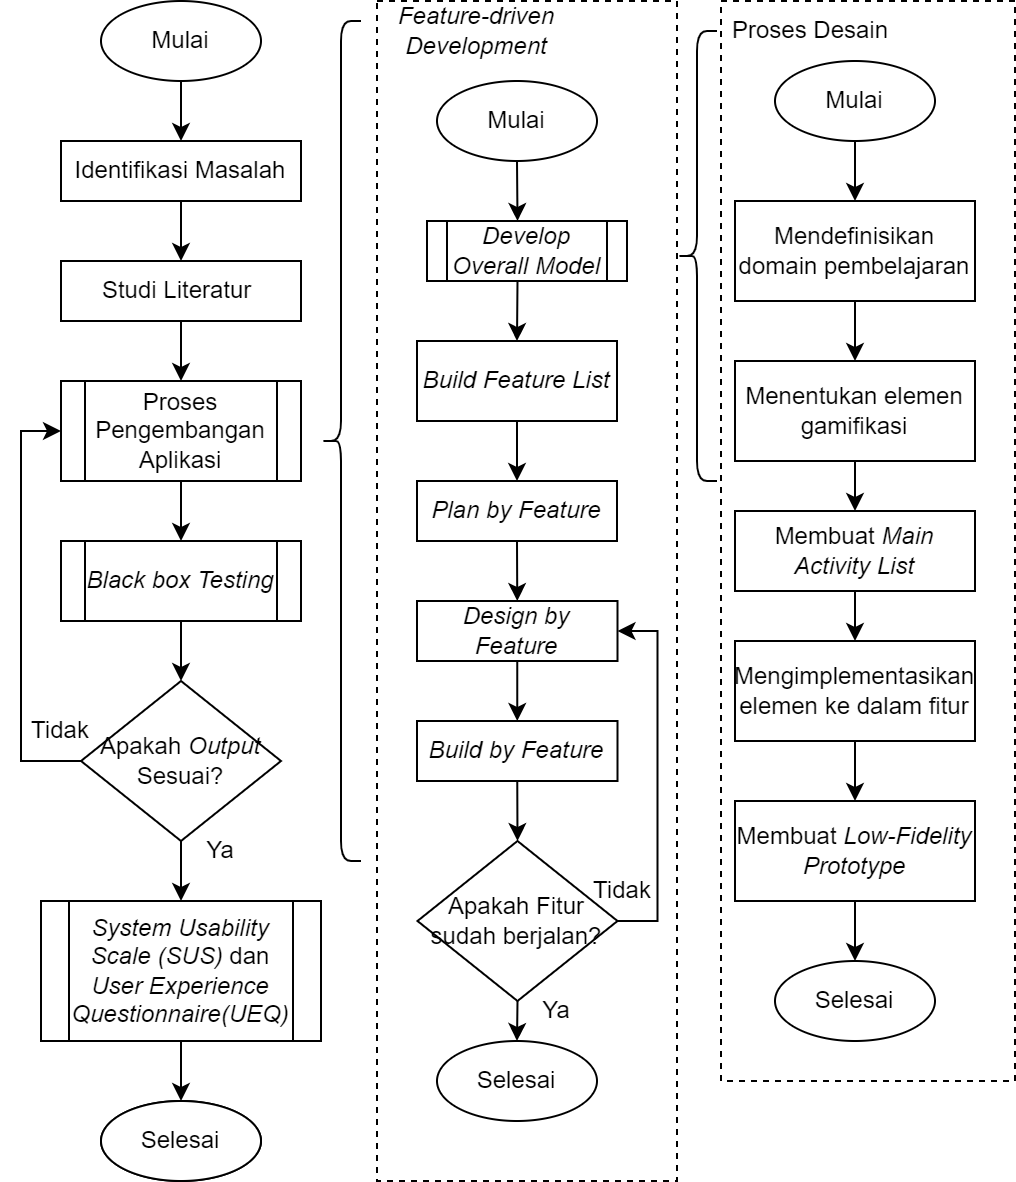
\includegraphics[width=\textwidth-1cm]{contents/chapter-3/images/Alur-tugas-akhir-2.png}
	\caption{Alur Tugas Akhir}
	\label{Fig:Alur Tugas Akhir}
\end{figure}
% \section{Etika, Masalah, dan Keterbatasan Penelitian (Opsional)}
\subsection{Identifikasi Masalah}
Secara keseluruhan, penelitian ini akan membahas mengenai sebuah pembelajaran dalam sebuah ilmu yang spesifik, yaitu ilmu tentang \textit{Clinical Decision Support System}.
Hal yang pertama dilakukan dalam penelitian ini ialah mengidentifikasi masalah yang dihadapi sebagai motivasi awal penulis untuk melakuakn penelitian.
Identifikasi masalah dengan cara observasi mengenai masalah yang dihadapi dalam sebuah pembelajaran. 	

Observasi yang dilakukan ialah dengan mencari jurnal dan fakta terkait proses pembelajaran dan hubungannya dengan efektivitas pembelajaran.
Dalam penemuannya, salah satu masalah yang masih dihadapi dari sebuah proses pembelajaran ialah mengenai efektivitas pembelajaran yang dipengaruhi oleh motivasi dan kesiapan mahasiswa atau siswa \cite{hasan2021media}.
Pada sumber yang sama juga dijelaskan bahwa salah satu upaya untuk meningkatkan efektivitas sebuah pembelajaran ialah dengan menggunakan sebuah media pembelajaran yang tepat.
Penjelasn tersebut dijelaskan pada buku yang ditulis oleh Hasan(2021) yang berjudul "Media Pembelajaran"\cite{hasan2021media}.
Tentu saja demikian, bagaimana kita dapat mendapatkan ilmu jika kita sendiri tidak memiliki keinginan untuk mendapatkannya.
Salah satu strategi dalam menangani masalah tersebut ialah implementasi \textit{game desain} pada media pembelajaran tersebut \cite{EnjoyLearningLikeGaming}, tapi tidak sembarang \textit{game elemen} dapat dimasukan ke dalam sebuah media pembelajaran.
Pemilihan \textit{game element} yang tepat merupakan aspek penting dalam pengembangan media pembelajaran yang efektif\cite{kapp2012gamification}. Pernyataan tersebut mengarahkan penulis pada sebuah pertanyaan "Bagaimana memilih \textit{game element} yang tepat untuk sebuah media pembelajaran".

Ilmu yang dibahas pada penelitian ini akan lebih spesifik pada ilmu \textit{Clinical Decision Support System}. Ilmu ini merupakan salah satu ilmu yang sedang populer dan potensinya sangat besar dalam dunia medis.
Ilmu ini tentu saja menarik untuk dipelajari mengingat potensinya yang besar dan masih bisa digali lagi, tapi masih belum ada media pembelajaran interaktif yang menyediakan pembelajaran mengenai ilmu ini.

Dari pernyataan-pernyataan tersebut, penulis dapat mengidentifikasi masalah yang dihadapi ialah media pembelajaran terkadang membosankan, dan hal tersebut akan berpengaruh ke dalam keefektivan pembelajran.
Selain itu, ilmu \textit{Clinical Decision Support System} belum menyediakan media pembelajran interaktif yang dapat menarik minat pengguna untuk mempelajarinya.
Dari masalah yang dihadapi, kemudian dapat dirumuskan kemungkinan solusi yang dapat menyelesaikan masalah tersebut. Salah satunya ialah dengan mengembangkan sebuah media pembelajaran yang secar spesifik membahas mengenai \textit{Clinical Decision Support System}.
Tidak samapai di sana, tentu saja media pembelajaran yang dikebangakan perlu memperhatikan faktor utama dari sebauh pembelajaran yaitu keefektivan pembelajaran.

\subsection{Studi Literatur}
Proses studi literatur pada penelitian ini dilakukan dengan tujuan untuk memperluas pemahaman mengenai isu yang serupa yang terjadi di lokasi lain, 
solusi pengembangan desain yang telah diimplementasikan oleh peneliti lain, serta implementasui gamifikasi yang melibatkan pemahaman tentang berbagai aspek, 
mulai dari jenis domain pembelajaran atau \textit{Type of Knowledge} hingga \textit{Framework} yang digunakan. 
Hal ini dilakukan melalui pembelajaran teori-teori, telaah buku, jurnal, dan sumber informasi lainnya yang relevan. 
Informasi yang diperoleh dari studi literatur tersebut akan menjadi dasar pertimbangan dalam mengembangkan fitur-fitur yang tepat untuk mengatasi masalah yang ada.
\subsection{\textit{Develop Overall Model}}
Setelah menelaaah literatur yanga ada, dilanjutkan dengan proses pengembangan. Proses pengembangan aplikasi ini dimulai dari mendesain model keseluruhan untuk sebuah aplikasi pembelajaran.
Sebelum melakukan proses desain, penulis akan menentukan domain ilmu yang akan dipelajari dalam sebuah media pembelajaran yang akan dikembangkan. Hal ini dimaksudkan untuk mempermudah untuk menetapkan elemen gamifikasi pada aplikasi tersebut.

Pegembangan media pembeljaran pada penelitian ini akan menggunakan kategori domain \textit{Declarative Knowledge}. Kategori ini cocok untuk ilmu \textit{Clinical Decision Support System} karena kategori ini mencakup pengetahuan tentang konsep-konsep dasar mengenai CDSS, seperti definisi CDSS, komponen-komponennya, prinsip-prinsip desain, dan metode evaluasi.
yang berhubungan dengan pengetahuan yang berkaitan dengan fakta, informasi, atau konsep yang dapat dinyatakan dengan jelas cocok untuk pengguna awam yang ingin memahami ilmu ini. Dalam CDSS, pengetahuan deklaratif mencakup pengetahuan medis dan informasi terkait yang digunakan untuk mendukung pengambilan keputusan klinis.

\subsubsection{\textit{User persona}}
Sebelum melakukan proses desain, akan dibuat terlebih dahulu sebuah \textit{user persona} dari gambaran umum aplikasi yang akan dibuat.
\textit{User persona} adalah representasi fiktif dari pengguna ideal atau target yang dibuat berdasarkan analisis dan pemahaman tentang karakteristik, kebutuhan, dan tujuan pengguna yang sebenarnya. 
Pembuatan \textit{user persona} adalah untuk membantu dalam memahami target dan membantu dalam merancang pengalaman pengguna yang lebih relevan dan efektif.
Dalam penelitian ini, \textit{user persona} dibuat berdasarkan informasi yang didapatkan melalui wawancara salah satu target audiense yaitu selaku mahasiswa yang sudah pernah mempelajari \textit{Clinical Decision Support System}.

Wawancara dilakukan secara tatap muka bertempat di Universitas Gadjah Mada. Narasumber bernama Zafira Farhani yang saat ini adalah seorang mahasiswa teknik biomedis.
Wawancara berlangsung kurang lebih selama 1 jam membicarakan mengenai mata kuliah yang pernah diambil oleh narasumber mengenai \textit{Clinical Decision Support System}.
Informasi yang dicari antara lain adalah pengalaman narasumber selama mempelajari mata kuliah tersebut, dan keinginan narasumber yang dapat membantu memahami mata kuliah tersebut.

\begin{figure}[H]
	\centering
	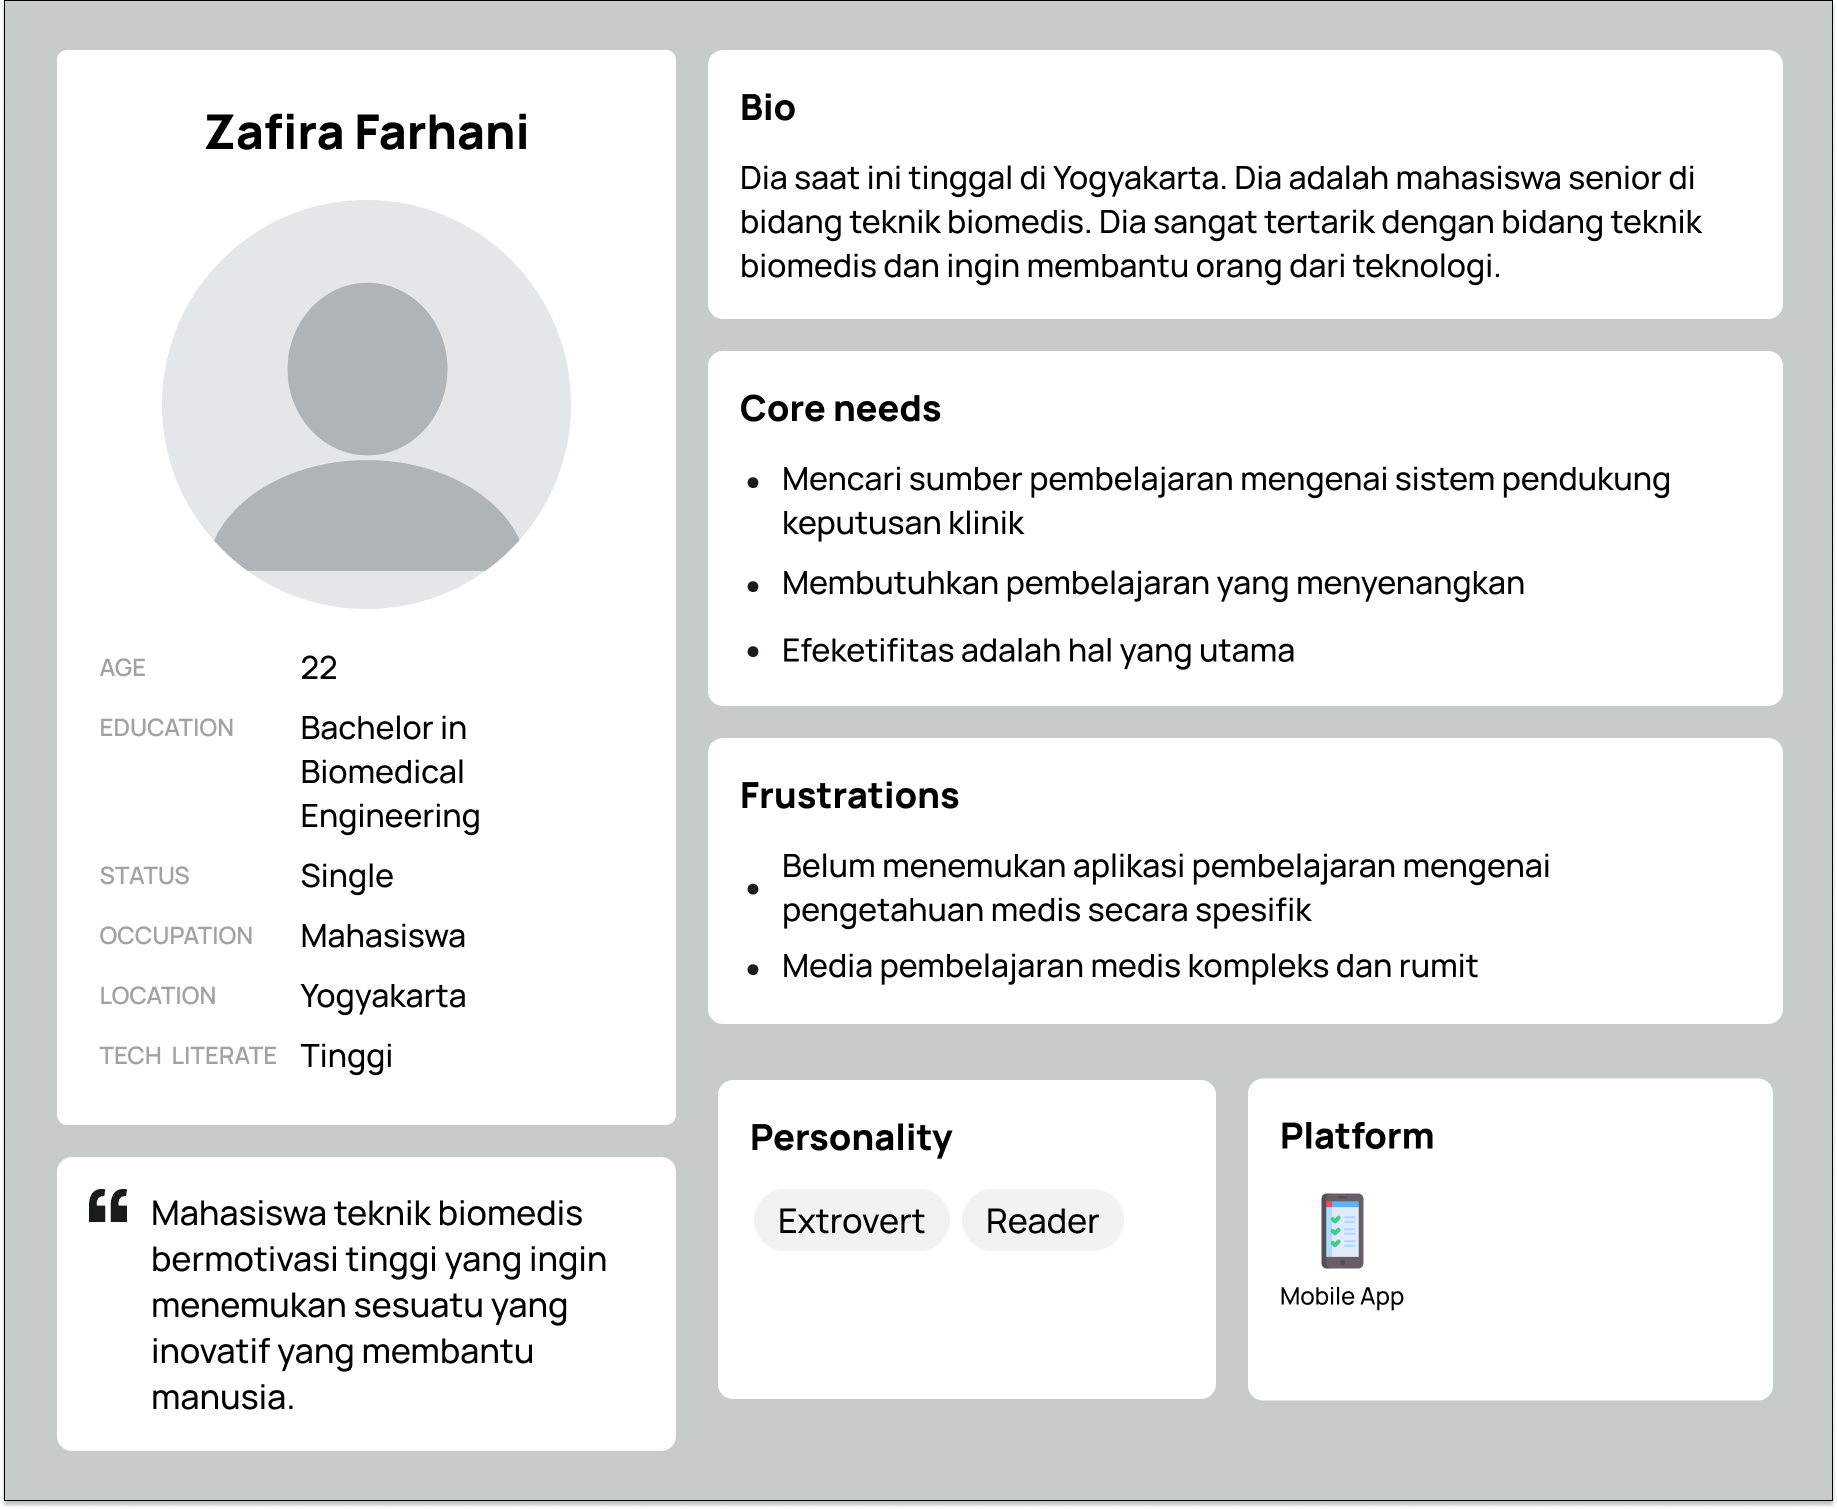
\includegraphics[width=\textwidth]{contents/chapter-3/images/up-dummy.png}
	\caption{\textit{User Persona}}
	\label{Fig:UserPersona}
\end{figure}

\subsubsection{\textit{Activity-centered Design}}
\begin{table}[H]
	\centering
	\caption{Struktur aktivitas utama}
	\begin{tabular}{|m{1cm}|m{0.9\textwidth}|}
		\hline
		\centering \textbf{ID} & \multicolumn{1}{c|}{\centering \textbf{Aktivitas Utama}}\\
		\hline
		A-01 & \textit{Google Sign-in} \\
		\hline
		A-02 & Melihat \textit{dashboard} halaman utama\\
		\hline
		A-03 & Mempelajari materi\\
		\hline
		A-04 & Mengerjakan kuis singkat mengnai materi \\
		\hline
		A-05 & Melihat urutan \textit{Leaderboard} dari kuis terkait\\
		\hline
		A-06 & Melihat penghargaan atau \textit{Achievement} berdasarkan kuis terkait \\
		\hline
		A-07 & \textit{Log-Out}\\
		\hline
	\end{tabular}
	\label{Tab: Tabel Main Activity}
\end{table}
Tabel \ref*{Tab: Tabel Main Activity} merupakan daftar aktivitas utama untuk aplikasi yang akan dikembangkan.
Secara keseluruhan aplikasi pembelajaran yang akan dikembangakan memiliki tujuan untuk mempelajari \textit{Clinical Decision Support System}. 
Aktivitas utama tersebut diformulasikan berdasrkan \textit{user persona}yang sudah dibuat. Aktivitas utama terdiri mempelajari materi, dan melakukan kuis untuk melatih pemahaman.
Dari daftar aktivitas tersebut, kemudian dirancang sebuah \textit{Use Case Diagram} sebagai gambaran umum perancangan aplikasi yang akan dikembangkan. \textit{Use Case Diagram} ditunjukkan pada gambar \ref*{Fig:Use Case Diagram}. 
\begin{figure}[H]
	\centering
	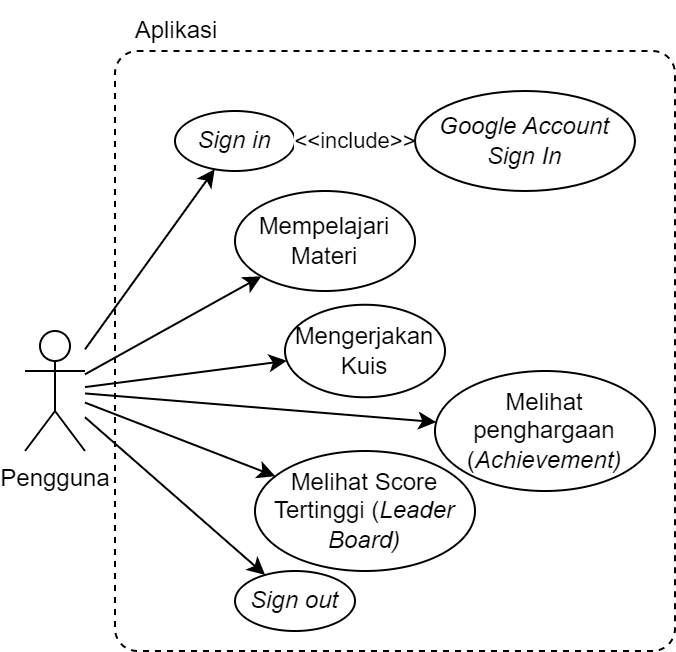
\includegraphics[width=0.7\textwidth]{contents/chapter-3/images/Use-Case-Diagram.png}
	\caption{\textit{Use Case Diagram}}
	\label{Fig:Use Case Diagram}
\end{figure}

\subsubsection{\textit{Gamification Design}}
Proses pengembangan gamifikasi dalam aplikasi ini akan didasari oleh kategori domain pembelajaran atau \textit{Type of Knowledge} ilmu yang diimplementasikan. Seperti yang sudah dijelasakan sebelumnya, domain pembelajaran ilmu \textit{Clinical Decision Support System} yang akan dikembangakan ialah kategori \textit{Declarative Knowledge}.
Dalam buku yang ditulis oleh Kapp(2012), setiap domain pembelajaran memiliki elemen gamifikasinya masing-masing. Dalam bukunya juga menjelaskan domain \textit{Declarative Knowledge} memiliki elemen gamifikasi \textit{Story/Narrative}, \textit{Sorting}, \textit{Matching}, dan \textit{Replayability}.
Lebih lengkapnya pada tabel \ref*{Tab:Declarative-knowledge}
\begin{table}[H]
	\centering
	\caption{Domain \textit{Declarative Knowledge}}
	\begin{tabular}{|p{2.7cm}|p{3cm}|p{2.7cm}|p{2.7cm}|p{2cm}|}
		\hline
		\centering\textbf{Domain Pembelajaran} &\centering\textbf{Definisi}  &\centering\textbf{Strategi Instruksi}  &\centering\textbf{Elemen Gamifikasi} &\multicolumn{1}{m{2cm}|}{\centering \textbf{Contoh}}\\
		\hline
		\textit{Declarative Knowledge} 
		&Asosiasi antara dua atau lebih objek. Ini biasanya berupa fakta, istilah khusus, dan singkatan. Kontennya harus dihafal.
		&Elaborasi, Pengorganisasian, Asosiasi, Pengulangan
		&\textit{Story/Narrative}, \textit{Sorting}, \textit{Matching}, dan \textit{Replayability}
		&\textit{Trivia, Hang-man, Drag and Drop} \\
		\hline
	\end{tabular}
	\label{Tab:Declarative-knowledge}
\end{table}
Dari hubungan tersebut, elemen gamifikasi yang akan digunakan ialah \textit{Story/Narrative} dan akan dikemas dalam bentuk materi yang dapat diakses secara berurutan mengenai \textit{Clinical Decision Support System}. Selain itu, elemen tersebut dapat dikemas dalam sebuah kuis singkat untuk menguji pemahaman.
Kuis yang dikembangkan dapat dikerjakan secara berulang ulang sehingga sesuai dengan elemen gamifikasi \textit{Replayability}. Kedua elemen ini, ialah elemen utama yang kemudian akan dikembangkan lagi dalam kerangka kerja gamifikasi.

Proses pengembangan gamifikasi akan menggunkan pendekatan kerangka kerja desain permainan \textit{MDA} yang terdiri dari \textit{Mechanics, Dynamics, and Aesthetics}. 
Pendekatan ini akan mengimplementasikan elemen permainan ke dalam produk penelitain ini, yaitu aplikasi pembelajaran.
Penggunaan metode dan rancangan ini disesuaikan dengan kebutuhan dan tujuan adanya gamifikasi dalam aplikasi yang dikembangkan.
Acuan pengembangan desain ini akan mengikuti dengan Aktivitas Utama yang sudah dirumuskan sebelumnya pada tabel \ref*{Tab: Tabel Main Activity}.
Pengembangan ini dimulai dari pengembangan \textit{Game Mechanics}.

\textit{Game Mechanics} berfokus pada aturan pada peraturan pada permainan. Mekanika permainan yang tersusun pada aplikasi ini ialah :
\begin{description}
	\item[\textit{Modes}]
	pada aplikasi, akan tedapat 2 mode, yaitu pembelajaran materi dan Kuis.
	Pembelajaran materi melibatkan materi-materi dasar mengenai \textit{Clinical Decision Support System}. Pengguna dapat membaca materi secara berurutan dimulau dari konsep umum \textit{DSS},\textit{CDSS}, \textit{Medical Diagnostic Test}, dan \textit{Electronic Health Record}.
	Selain itu ada mode kuis yang
	merupakan elemen mekanik yang melibatkan pertanyaan dan jawaban. Pengguna dapat menguji pengetahuan mereka dan mendapatkan poin atau penghargaan berdasarkan hasil kuis yang mereka jawab dengan benar.
	\item[\textit{Points}] merupakan elemen mekanik yang digunakan untuk memberikan insentif kepada pengguna dalam menyelesaikan tugas atau mencapai tujuan tertentu. Poin dapat diberikan berdasarkan aktivitas atau pencapaian tertentu dalam aplikasi.
	\item[\textit{Achievement}] merupakan elemen mekanik yang memberikan penghargaan kepada pengguna ketika mereka mencapai tujuan atau melakukan pencapaian tertentu dalam aplikasi. Pencapaian ini dapat berupa sertifikat, badge, atau level yang diberikan kepada pengguna sebagai bentuk pengakuan atas prestasi mereka.
	\item[\textit{Time Attack}] Merupakan elemen mekanik yang akan diimplementasikan pada fitur kuis. Elemen ini akan memberikan tantangan kepada pengguna untuk mengerjakan kuis dengan waktu yang ditentukan. Waktu pengerjaan ini juga akan memperngaruhi poin yang didapatkan oleh pengguna.
\end{description}
Setelah selesai mendesain mekanika permainan, dilanjutkan dengan mendesain dinamika permainan. \textit{Dynamics} atau Dinamika merujuk pada perilaku sistem permainan yang timbul dari interaksi antara pemain dengan mekanika permainan. Ini mencakup respons terhadap tindakan pemain, aliran permainan, pola interaksi, dan perubahan yang terjadi seiring permainan berlangsung. Dinamika permainan yang tersusun pada aplikasi ini ialah : 
\begin{description}
	\item[{Materi dan kuis yang diakses berurutan}] merupakan elemen dinamis yang melibatkan pengguna dalam mengeksplorasi dan memperoleh pengetahuan secara berurutan. Pengguna dapat menavigasi melalui materi yang disusun dengan urutan tertentu untuk memahami konten aplikasi secara sistematis.
	\item[\textit{Leaderboard}] Merupakan elemen dinamis yang memungkinkan pengguna untuk melihat peringkat mereka dan peringkat pengguna lain dalam aplikasi. Ini menciptakan dinamika persaingan di antara pengguna, mendorong mereka untuk mencapai skor tinggi dan berada di peringkat teratas.
\end{description}
Akhir dari kerangka kerja ini kemudian dilanjutkan dengan mendesain estetika permainan. \textit{Aesthetics} atau estetika merujuk pada perasaan, emosi, dan kepuasan yang dirasakan oleh pemain saat bermain. Estetika memberikan dimensi pengalaman permainan yang melibatkan elemen seperti kegembiraan, kepuasan, kekaguman, dan tantangan. Estetika permainan yang tersusun pada aplikasi ini ialah : 
\begin{description}
	\item [\textit{Unlocking Part}] berdasarkan urutan, diharapkan pengguna mendapatkan perasaan untuk membuka materi baru.
	\item [\textit{On Boarding}] sebagai panduan kepada pengguna baru untuk membantu pengguna mengikuti dinamika permainan yang dibuat.
	\item [\textit{Desain Visual}] sebagai elemen antarmuka yang melibatkan tampilan dan estetika aplikasi. Desain visual yang menarik dan konsisten dapat meningkatkan pengalaman pengguna dan membuat aplikasi lebih menarik.
\end{description}
Setelah mendesain keseluruhan gamifikasi, proses selanjutnya ialah menuliskan daftar fitur yang akan diimplementasikan dalam aplikasi yang dikembangkan.
Penulisan daftar fitur ini tentunya merupakan fitur yang sudah dimodifikasi dengan elemen gamifikasi 
atau bisa disebut dengan pengembangan aktivitas utama yang sudah melalui proses gamifikasi.
\subsection{\textit{Build Feature List}}
Proses \textit{Build Feature List} akan menuliskan daftar fitur yang dikembangkan dari desain gamifikasi yang sudah dibuat.
Daftar-daftar yang akan dijelaskan ini adalah perkembangan aktivitas yang lebih detail dari aktivitas utama pada tabel \ref*{Tab: Tabel Main Activity}.
Dengan demikian, fitur aktivitas utama akan menjadi kelompok fitur set yang memiliki bagian-bagian fitur lainnya.
\begin{table}[H]
	\centering
	\caption{Daftar Fitur}
	\begin{tabular}{|m{3cm}|p{0.68\textwidth}|m{1cm}|}
		\hline
		\centering\textbf{Aktivitas Utama} & \centering\textbf{Fitur} & \multicolumn{1}{m{1cm}|}{\centering \textbf{ID}} \\
		\hline
		\multirow{4}{2.5cm}{\textit{Sign-in}} &Menampilkan halaman \textit{Sign-in} & F-01 \\
		\cline{2-3}
		 &Mencatat \textit{user} baru ketika melakukan \textit{Sign-in} pertama & F-02 \\
		\cline{2-3}
		 &Aplikasi dapat memberikan akses pengguna ketika pengguna sudah terdaftar& F-03 \\
		\hline
		\multirow{5}{2.5cm}{Melihat \textit{dashboard} halaman utama} &Menampilkan halaman \textit{On Boarding} jika \textit{user} belum terdaftar & F-04 \\
		\cline{2-3}
		&Menampilkan halaman utama aplikasi& F-05 \\
		\cline{2-3}
		&Menampilkan \textit{side drawer}& F-06 \\
		\cline{2-3}
		&\textit{Dialog box Sign Up} jika memilih fitur, tapi \textit{user} belum terdaftar& F-07 \\
		\cline{2-3}
		&Memilih fitur kuis, materi, dan profil& F-08 \\
		\hline
		\multirow{6}{2.5cm}{Mempelajari materi} &Menampilkan halaman daftar materi yang tersedia& F-09 \\
		\cline{2-3}
		&Menampilkan materi yang dipilih & F-10 \\
		\cline{2-3}
		&Keluar dari materi yang dipilih& F-11 \\
		\cline{2-3}
		&Fitur kunci materi jika materi sebelumnya belum dibaca& F-12 \\
		\cline{2-3}
		&Keluar dari halaman daftar materi dan kembali ke halaman utama& F-13 \\
		\hline

	\end{tabular}
\end{table}

\newpage
\begin{table}[H]
	\begin{tabular}{|m{3cm}|p{0.68\textwidth}|p{1cm}|}
		\hline
		\centering\textbf{Aktivitas Utama} & \centering\textbf{Fitur} & \multicolumn{1}{m{1cm}|}{\centering \textbf{ID}} \\
		\hline
		\multirow{7}{2.5cm}{Mengerjakan kuis singkat mengnai materi} &Menampilkan halaman daftar kuis& F-14 \\
		\cline{2-3}
		&Menampilkan halaman kuis yang dipilih& F-15 \\
		\cline{2-3}
		&Memilih salah satu jawaban kuis berbasis pilihan ganda& F-16 \\
		\cline{2-3}
		&Menampilkkan halaman kuis nomor selanjutnya& F-17 \\
		\cline{2-3}
		&Menampilkan halaman kuis nomor sebelumnya& F-18 \\
		\cline{2-3}
		&Menampilkan ringkasan kuis& F-19 \\
		\cline{2-3}
		&Menyelesaikan kuis& F-20 \\
		\hline
		\multirow{8}{2.5cm}{Mengerjakan kuis singkat mengnai materi} &Menampilkan halaman daftar materi& F-21 \\
		\cline{2-3}
		&Mendapatkan skor kuis& F-22 \\
		\cline{2-3}
		&Mencatat skor kuis& F-23 \\
		\cline{2-3}
		&Menampilkan warna merah untuk jawaban yang salah dan warna hijau untuk jawaban yang benar dalam ulasan kuis& F-24 \\
		\cline{2-3}
		&Memeriksa 1 per 1 jawaban kuis setelah mendapatkan skor& F-25 \\
		\cline{2-3}
		&Mengerjakan kembali kuis& F-26 \\
		\cline{2-3}
		&Menutup halaman kuis dan kembali ke halaman daftar kuis& F-27 \\
		\cline{2-3}
		&Menutup halaman daftar kuis dan kembali ke halaman utama& F-28 \\
		\hline
		\multirow{3}{3cm}{Melihat urutan \textit{Leaderboard} dari kuis terkait} &Menampilkan halaman \textit{Leaderboard} untuk kuis yang dipilih & F-29 \\
		\cline{2-3}
		&Menampilkan hasil skor kuis pribadi yang sudah dikerjakan& F-30 \\
		\cline{2-3}
		&Menampilkan urutan skor dari yang tertinggi hingga terendah& F-31 \\
		\cline{2-3}
		&Menutup halaman leaderboard dan kembali ke halaman daftar kuis& F-32\\
		\hline
		\multirow{4}{3cm}{Melihat penghargaan atau \textit{Achievement} berdasarkan kuis terkait} &Menampilkan halaman profil& F-33 \\
		\cline{2-3}
		&Menampilkan penghargaan yang ada dalam halaman profil& F-34 \\
		\cline{2-3}
		&Menampilkan hasil scroe dari setiap kuis yang sudah dikerjakan& F-35 \\
		\cline{2-3}
		&Menutup halaman profil dan kembali ke halaman utama aplikasi& F-36 \\
		\hline
		\multirow{1}{2.5cm}{\textit{Log-Out}} &Menghentikan pemberian akses pengguna ketika pengguna sudah terdaftar& F-37 \\
		\hline
	\end{tabular}
\end{table}
\subsection{\textit{Plan by Feature}}
Proses ini adalah perencanaan pengembangan atau proses mbentuk \textit{project timeline} dari seluruh fitur pada setiapfeature set seperti yang terlihat pada Tabel.
Perancangan ini bertujuan untuk menetapkan estimasi waktu agar proses pengembangan tidak tertinggal jauh.
Proses pengembangan dilakukan secara bertahap fitur demi fitur. Tanggal pengembangan dimulai dari awal maret hingga bulan mei, sekitar kurang lebih 3 bulan.

\begin{table}[H]
	\begin{tabular}{|p{3cm}|p{0.62\textwidth}|p{2cm}|}
		\hline
		\centering\textbf{\textit{Feature Set}} & \centering\textbf{Fitur} & \multicolumn{1}{m{2cm}|}{\centering \textbf{Tanggal}} \\
		\hline
		\multirow{3}{2.5cm}{\textit{Sign-in}} &Menampilkan halaman Sign-in & \multirow{3}{2cm}{13 Marert - 14 Maret} \\
		\cline{2-2}
		 &Mencatat \textit{user} baru ketika melakukan \textit{Sign-in} pertama & \\
		\cline{2-2}
		 &Aplikasi dapat memberikan akses pengguna ketika pengguna sudah terdaftar&  \\
		\hline
		\multirow{1}{2.5cm}{\textit{Log-Out}} &Menghentikan pemberian akses pengguna ketika pengguna sudah terdaftar& 13 Maret - 14 Maret \\
		\hline
		\multirow{14}{2.5cm}{Mengerjakan kuis singkat mengenai materi} &Menampilkan halaman daftar kuis& \multirow{14}{2cm}{15 Maret - 10 April}\\
		\cline{2-2}
		&Menampilkan halaman kuis yang dipilih& \\
		\cline{2-2}
		&Memilih salah satu jawaban kuis berbasis pilihan ganda&  \\
		\cline{2-2}
		&Menampilkkan halaman kuis nomor selanjutnya&  \\
		\cline{2-2}
		&Menampilkan halaman kuis nomor sebelumnya& \\
		\cline{2-2}
		&Menampilkan ringkasan kuis& \\
		\cline{2-2}
		&Menyelesaikan kuis&\\
		\cline{2-2}
		&Mendapatkan skor kuis&  \\
		\cline{2-2}
		&Mencatat skor kuis&  \\
		\cline{2-2}
		&Menampilkan warna merah untuk jawaban yang salah dan warna hijau untuk jawaban yang benar dalam ulasan kuis& \\
		\cline{2-2}
		&Memeriksa 1 per 1 jawaban kuis setelah mendapatkan skor&  \\
		\cline{2-2}
		&Mengerjakan kembali kuis& \\
		\cline{2-2}
		&Menutup halaman kuis dan kembali ke halaman daftar kuis&  \\
		\cline{2-2}
		&Menutup halaman daftar kuis dan kembali ke halaman utama& \\
		\hline
		
	\end{tabular}
\end{table}
\newpage
\begin{table}[H]
	\begin{tabular}{|m{3cm}|p{0.62\textwidth}|p{2cm}|}
		\hline
		\centering\textbf{\textit{Feature Set}} & \centering\textbf{Fitur} & \multicolumn{1}{m{2cm}|}{\centering \textbf{Tanggal}} \\
		\hline
		\multirow{5}{2.5cm}{Melihat \textit{dashboard} halaman utama} &Menampilkan halaman \textit{On Boarding} jika \textit{useer} belum terdaftar &\multirow{5}{2cm}{11 April - 22 April}\\
		\cline{2-2}
		&Menampilkan halaman utama aplikasi&  \\
		\cline{2-2}
		&Menampilkan \textit{side drawer}&  \\
		\cline{2-2}
		&\textit{Dialog box Sign Up} jika memilih fitur, tapi \textit{user} belum terdaftar&  \\
		\cline{2-2}
		&Memilih fitur kuis, materi, dan profil&  \\
		\hline
		\multirow{4}{2.5cm}{Melihat urutan \textit{Leaderboard} dari kuis terkait} &Menampilkan halaman \textit{Leaderboard} untuk kuis yang dipilih & \multirow{4}{2cm}{22 April - 30 April} \\
		\cline{2-2}
		&Menampilkan hasil skor kuis pribadi yang sudah dikerjakan&  \\
		\cline{2-2}
		&Menampilkan urutan skor dari yang tertinggi hingga terendah&  \\
		\cline{2-2}
		&Menutup halaman leaderboard dan kembali ke halaman daftar kuis&  \\
		\hline
		\multirow{5}{2.5cm}{Mempelajari materi} &Menampilkan halaman daftar materi yang tersedia& \multirow{6}{2.5cm}{30 April - 5 Mei} \\
		\cline{2-2}
		&Menampilkan materi yang dipilih &  \\
		\cline{2-2}
		&Keluar dari materi yang dipilih&  \\
		\cline{2-2}
		&Fitur kunci materi jika materi sebelumnya belum dibaca&  \\
		\cline{2-2}
		&Keluar dari halaman daftar materi dan kembali ke halaman utama&  \\
		\hline
		\multirow{4}{3cm}{Melihat penghargaan atau \textit{Achievement} berdasarkan kuis terkait} &Menampilkan halaman profil& \multirow{4}{2cm}{5 Mei - 12 Mei} \\
		\cline{2-2}
		&Menampilkan penghargaan yang ada dalam halaman profil&  \\
		\cline{2-2}
		&Menampilkan hasil scroe dari setiap kuis yang sudah dikerjakan&  \\
		\cline{2-2}
		&Menutup halaman profil dan kembali ke halaman utama aplikasi&  \\
		\hline
	\end{tabular}
\end{table}
\newpage
\subsection{\textit{Design by Feature}}
Setelah menyusun daftar fitur dan merencanakan pengembangannya, selanjutnya adalah pembuatan design sesuai dengan perencangaan pengembangan.
Proses ini akan mengembangkan desain untuk setiap fitur yang akan dikembangkan dimulai dari \textit{Activity Diagram} sebagai acuan untuk pengembangan prototype. 
Lalu, dari \textit{Activity Diagram} tersebut dibuat prototype sebagai gambaran antarmuka aplikasi yang akan dikembangkan.
Prototype desain berupa \textit{Mid-Fidelity Wireframe}
\subsubsection{\textit{Feature set : Sign-in}}
\textbf{\textit{Activity Diagram}} pada gambar \ref*{Fig:ActivityDiagramSignIn} merupakan skenario yang dapat user lakukan ketika ingin melakukan \textit{log-in} pada aplikasi.
Proses \textit{log-in} pada aplikasi akan menggunakan \textit{Google Account Authentication} untuk mempermudah proses masuk agar tidak perlu mendaftarkan lagi pada aplikasi.
Scenario yang diterapkan ialah pada halaman \textit{Log-in} akan terdapat 1 tombol dengan tulisan \textit{"Sign in with Google"}, dan pengguna dapat masuk menggunakan autentikasi akun google yang dimiliki pengguna.
Kemudian,aplikasi akan mendeteksi apakah akun tersebut sudah terdaftar di database atau belum. Jika sudah, aplikasi akan langsung memberikan akses pada pengguna, jika belum aplikasi akan mencatat pengguna baryu ke dalam database.
\begin{figure}[H]
	\centering
	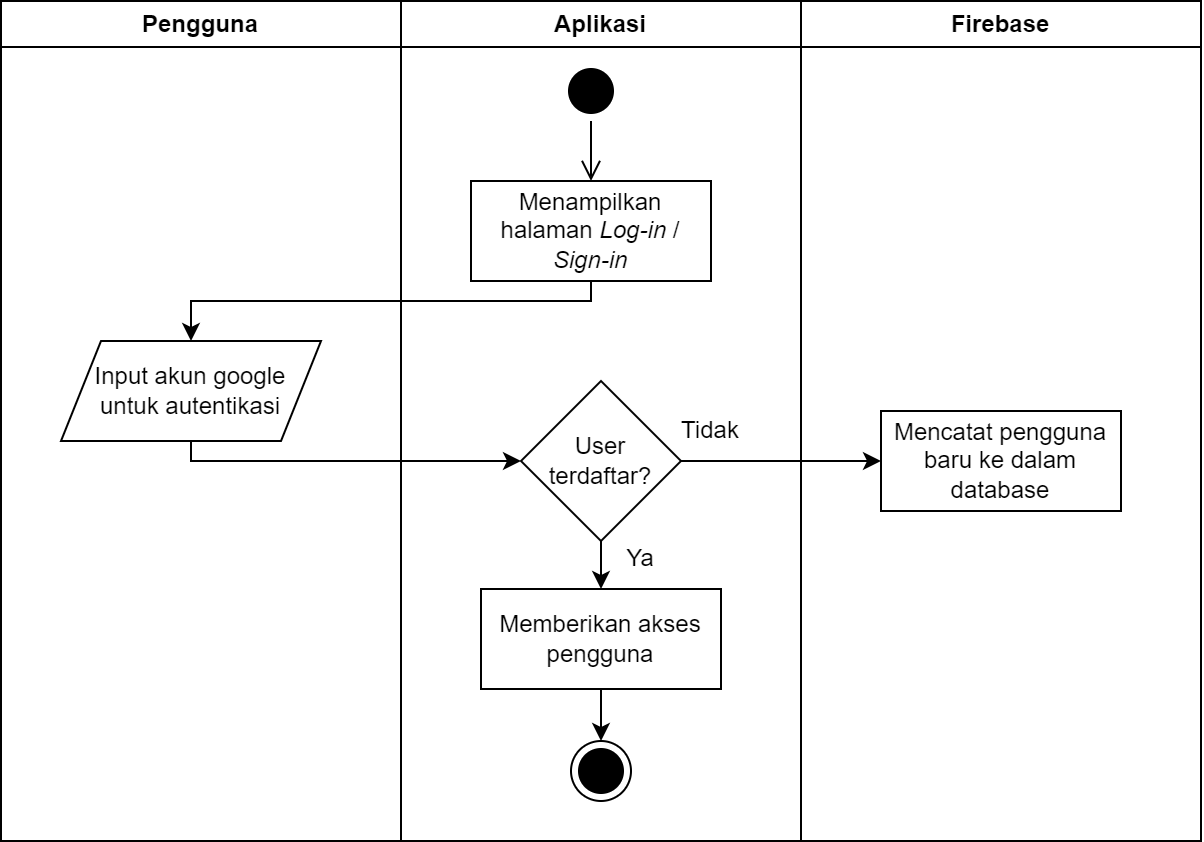
\includegraphics[width=0.8\textwidth]{contents/chapter-3/images/AD-signin.png}
	\caption{\textit{Sign-in Feature Set Activity Diagram}}
	\label{Fig:ActivityDiagramSignIn}
\end{figure}
Dari \textit{Activity Diagram} tersebut kemudian mengembangkan desain antarmuka atau \textbf{\textit{Prototype}} untuk halaman \textit{Log-in} seperti disematkan pada gambar \ref*{Fig:FeatureSetLogin}.
% Fitur ini tidak memiliki \textit{game mechanics} dalam pengembangannya, melainkan mengimplementasikan \textit{Aesthetics} untuk mengembangkan antarmuka yang menarik.
\begin{figure}[H]
	\centering
	\begin{subfigure}[b]{0.3\textwidth}
		\centering
	  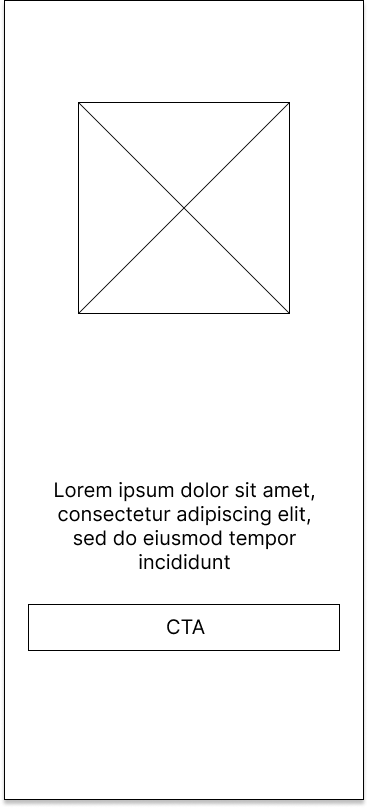
\includegraphics[width=\linewidth]{contents/chapter-3/images/MF-login.png}
	  \caption{Halaman utama \textit{Log-in}}
	  \label{fig:ActivityLogin}
	\end{subfigure}
	\begin{subfigure}[b]{0.3\textwidth}
		\centering
	  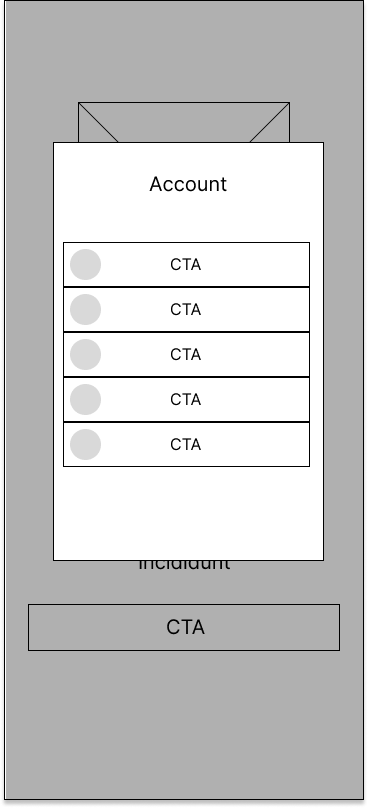
\includegraphics[width=\linewidth]{contents/chapter-3/images/MF-login-2.png}
	  \caption{Pilih akun \textit{Log-in}}
	  \label{fig:ActivityLogin2}
	\end{subfigure}
	\caption{\textit{Prototype} antarmuka halaman \textit{Log-in}}
	\label{Fig:FeatureSetLogin}
\end{figure}
Pada \textit{prototype} tersebut ada 2 halaman, yaitu halaman \textit{log-in} yang terdiri dari gambar, tulisan, dan sebuah tombol (gambar \ref*{fig:ActivityLogin}).
Sedangkan halaman 1 lagi adalah halaman pemilihan akun google yang akan dijadikan autentikasi pada aplikasi yang ditunjukkan pada gambar \ref*{fig:ActivityLogin2}

\subsubsection{\textit{Feature set : Dashboard}}
Halaman\textit{Dashboard} akan menjadi halaman pertama yang ditampilkan ketika pengguna sudah dapat mengakses aplikasi.
Untuk pengguna yang belum memiliki akses dan belum terdaftar pada \textit{database}, pengguna akan diarahkan ke halaman \textit{On Boarding} yang akan menampilkan sedikit informasi aplikasi yang sedang berjalan.
Halaman boarding akan terdiri dari 3 halaman dimana setiap halaman menampilkan objective dari aplikasi.
Pada halaman terakhir, ada sebuah tombol untuk masuk ke dalam aplikasi. Skenario aktivitas digambarkan oleh gambar \ref*{Fig:ActivityMain}
\begin{figure}[H]
	\centering
	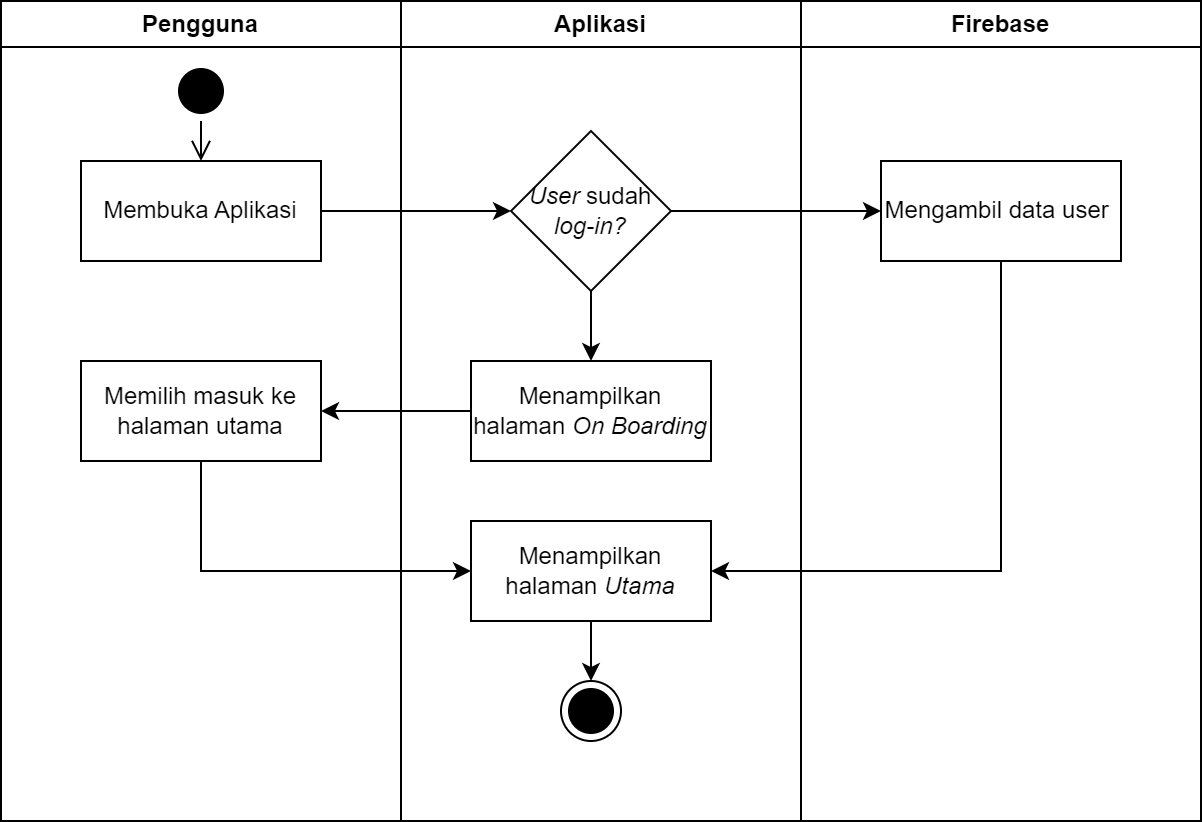
\includegraphics[width=0.8\textwidth]{contents/chapter-3/images/AD-halamanutama.png}
	\caption{User Persona}
	\label{Fig:ActivityMain}
\end{figure}
\textit{Prototype} halaman \textit{On Boarding} terdapat pada gambar \ref*{Fig:OnBoarding}. Pada tampilan \textit{prototype} akan terdapat sebuah gambar untuk menciptakan estetika permainan,
sebuah tulisan yang akan menuliskan objektif dari aplikasi, dan sebuah tombol untuk berpindah halaman.
\begin{figure}[H]
	\centering
	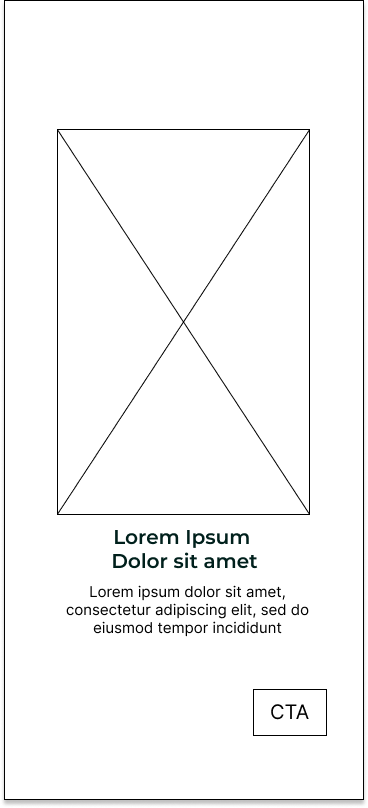
\includegraphics[width=0.3\textwidth]{contents/chapter-3/images/MF-Boarding.png}
	\caption{\textit{On Boarding}}
	\label{Fig:OnBoarding}
\end{figure}
\newpage
Fitur ini akan memberikan kesan dinamika yang akan dialami oleh pengguna, dan menambah kesan estetika permianan untuk menunjukkan aplikasinya kepada pengguna baru.
Selanjutnya, setalah halaman \textit{on boarding}, didesain juga halaman utama yang akan menjadi \textit{dashboard} dari aplikasi ini.
\textit{Dashboard} aplikasi ini akan menampilkan pilihan navigasi dari fitur yang disediakan. Diantaranya ialah fitur kuis, fitur materi, dan fitur profil. 
Fitur kuis dan materi akan ditampilkan pada halaman depan aplikasi halama utamanya, sedangkan profil akan disematkan pada \textit{side drawer} seperti pada gambar \ref*{fig:ActivityMain4}
\begin{figure}[H]
	\centering
	\begin{subfigure}[b]{0.3\textwidth}
		\centering
	  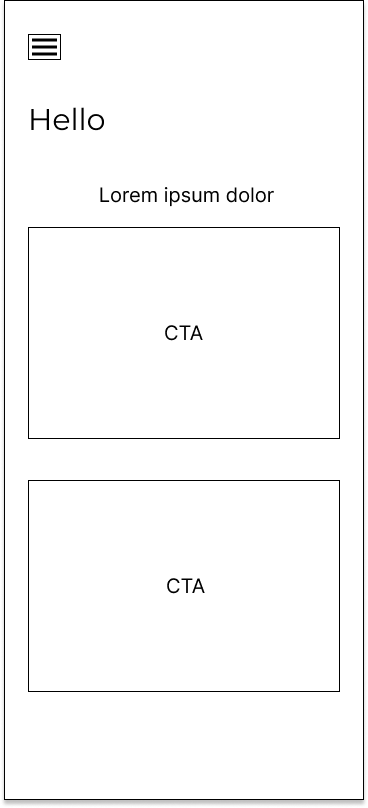
\includegraphics[width=\linewidth]{contents/chapter-3/images/MF-home.png}
	  \caption{Halaman utama}
	  \label{fig:ActivityMain2}
	\end{subfigure}
	\begin{subfigure}[b]{0.3\textwidth}
		\centering
	  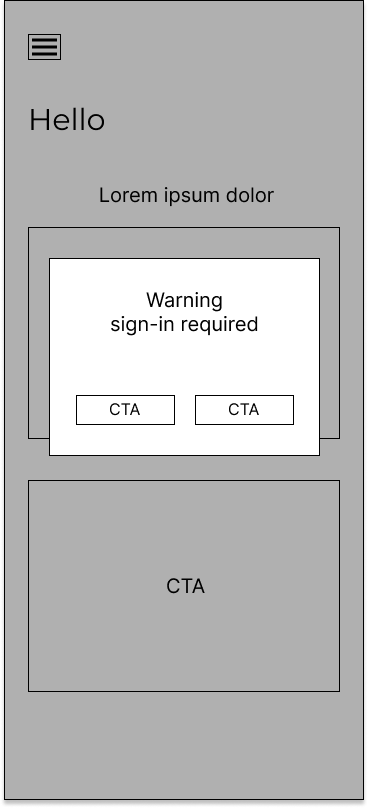
\includegraphics[width=\linewidth]{contents/chapter-3/images/MF-home-2.png}
	  \caption{\textit{Warning dialog}}
	  \label{fig:ActivityMain3}
	\end{subfigure}
	\begin{subfigure}[b]{0.3\textwidth}
		\centering
	  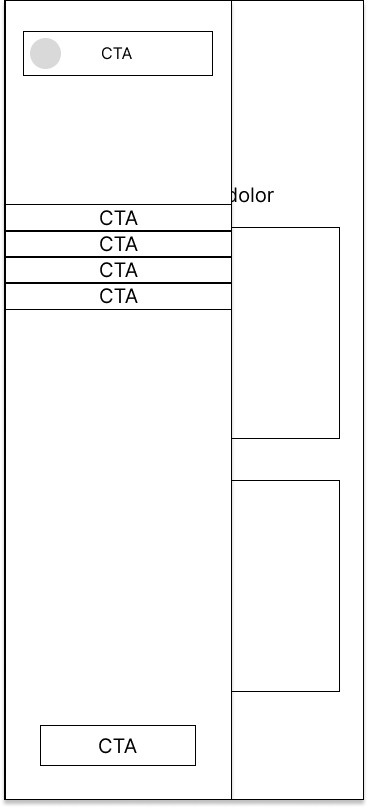
\includegraphics[width=\linewidth]{contents/chapter-3/images/MF-home-3.png}
	  \caption{\textit{Drawer}}
	  \label{fig:ActivityMain4}
	\end{subfigure}
	\caption{\textit{Prototype} antarmuka halaman \textit{Dashboard} utama}
	\label{Fig:FeatureSetDashboard}
\end{figure}
Pada halaman utama, jika pengguna belum melakukan \textit{sign-in}, pengguna akan diberikan \textit{warning dialog} seperti pada gambar \ref*{fig:ActivityMain3} untuk melakukan \textit{sign-in}.
\textit{Warning dialog} tersebut akan menampilkan 2 opsi tombol. Jika warning dialog diafirmasi, maka akan diarahkan ke halaman \textit{Sign-in}.
\subsubsection{\textit{Feature set : Log-out}}
Fitur \textit{Log-out} atau mengeluarkan akses aplikasi dari akun google merupakan fitur yang datang sejalan dengan fitur \textit{sign-in}.
Fitur ini memungkinkan kita mengeluarkan akun google kita dari aplikasi. Dalam pengembangan ini, fitur ini akan disematkan pada \textit{side drawer} bagian bawah aplikasi.
Jika pengguna sudah \textit{sign-in} dan ingin mengeluarkan akunnya dari aplikasi, pengguna bisa melakukan aktivitas seperti pada tabel \ref*{Fig:ActivityOut}
\begin{figure}[H]
	\centering
	\caption{\textit{Activity Diagram Log-out}}
	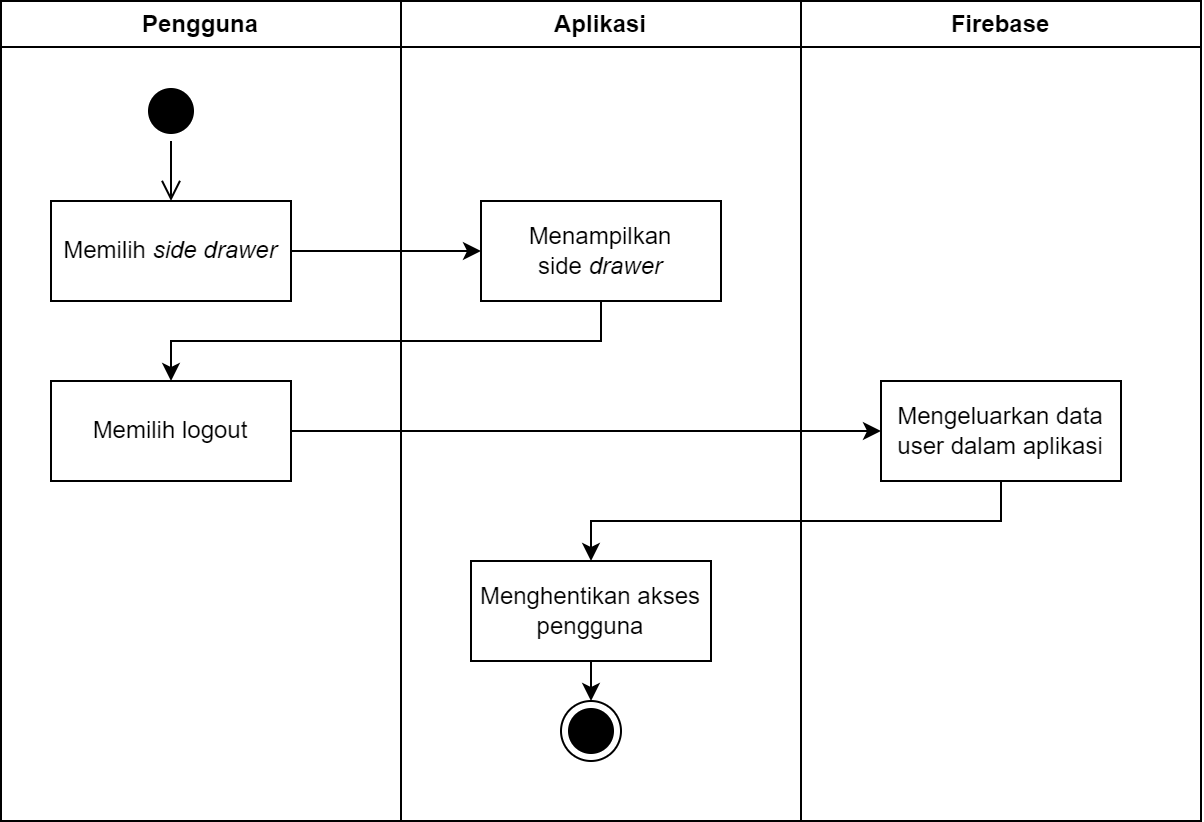
\includegraphics[width=0.8\textwidth]{contents/chapter-3/images/AD-signout.png}
	\label{Fig:ActivityOut}
\end{figure}
\subsubsection{\textit{Feature set : Quiz}}
Selanjutnya dikembangkan desain untuk fitur utama gamifikasi aplikasi ini, yaitu kuis singkat untuk meningkatkan pemahaman mengenai materi.
Kuis singkat ini akan terdiri dari paketan kuis yang di dalamnya terdapt sejumlah nomor yang dapat kita kerjakan. Kemudian pengguna akan memilih pilihan paling benar dari pertanyaan yang diberikan.
Jumlah soal pada pengembangan ini akan dibuat sebanyak 4 peket kuis dari 4 materi utama \textit{Clinical Decision Support System}. Diantaranya adalah konsep dasar \textit{Decision Support system}, \textit{Clinical Decision Support System}, \textit{Medical Diagnostic Test}, dan \textit{Electronic Health Record}.
Masing masing kuis akan terdiri dari 5 pertanyaan seputar materinya. Dalam menyusun soal, penulis menggunakan referensi dari materi mata kuliah \textit{Clinical Decision Support System}.

Skenario atau dinamika yang ditawarkan dalam fitur ini ialah pengguna dapat memilih salah 1 paket kuis untuk dikerjakan. Pengguna akan dihadapi oleh pertanyaan soal kuis dimulai nomor 1 hingga nomor terakhir.
Pengguna harus menjawab soal sesuai dengan pertanyaan yang disuguhkan. Semakin banyak jawaban benar, maka semakin banyak juga poin yang didapat. Pengguna dapat secara berurutan mengerjakan soal yang diberikan, dan pengguna juga bisa kembali ke nomor sebelumnya jika dirasa belum yakin.
Selain itu, dalam pengerjaannya pengguna dapat berpindah dari nomor 1 ke nomor lainnya dengan fitur \textit{overview}. Jika pengguna telah selesai mengerjakannya, pengguna dapat memeriksa kembali melalui fitur \textit{overview} tersebut pada akhir sesi kuis.
Lalu pengguna dapat menyelesaikan kuisnya dan mendapatkan poin. Poin akan secara otomatis tercatat pada \textit{database} akun yang terkait. Skenario digambarkan dalam \textit{Activity Diagram} pada gambar \ref*{fig:ActivityQuiz}


\newpage

\begin{figure}[H]
	\centering
	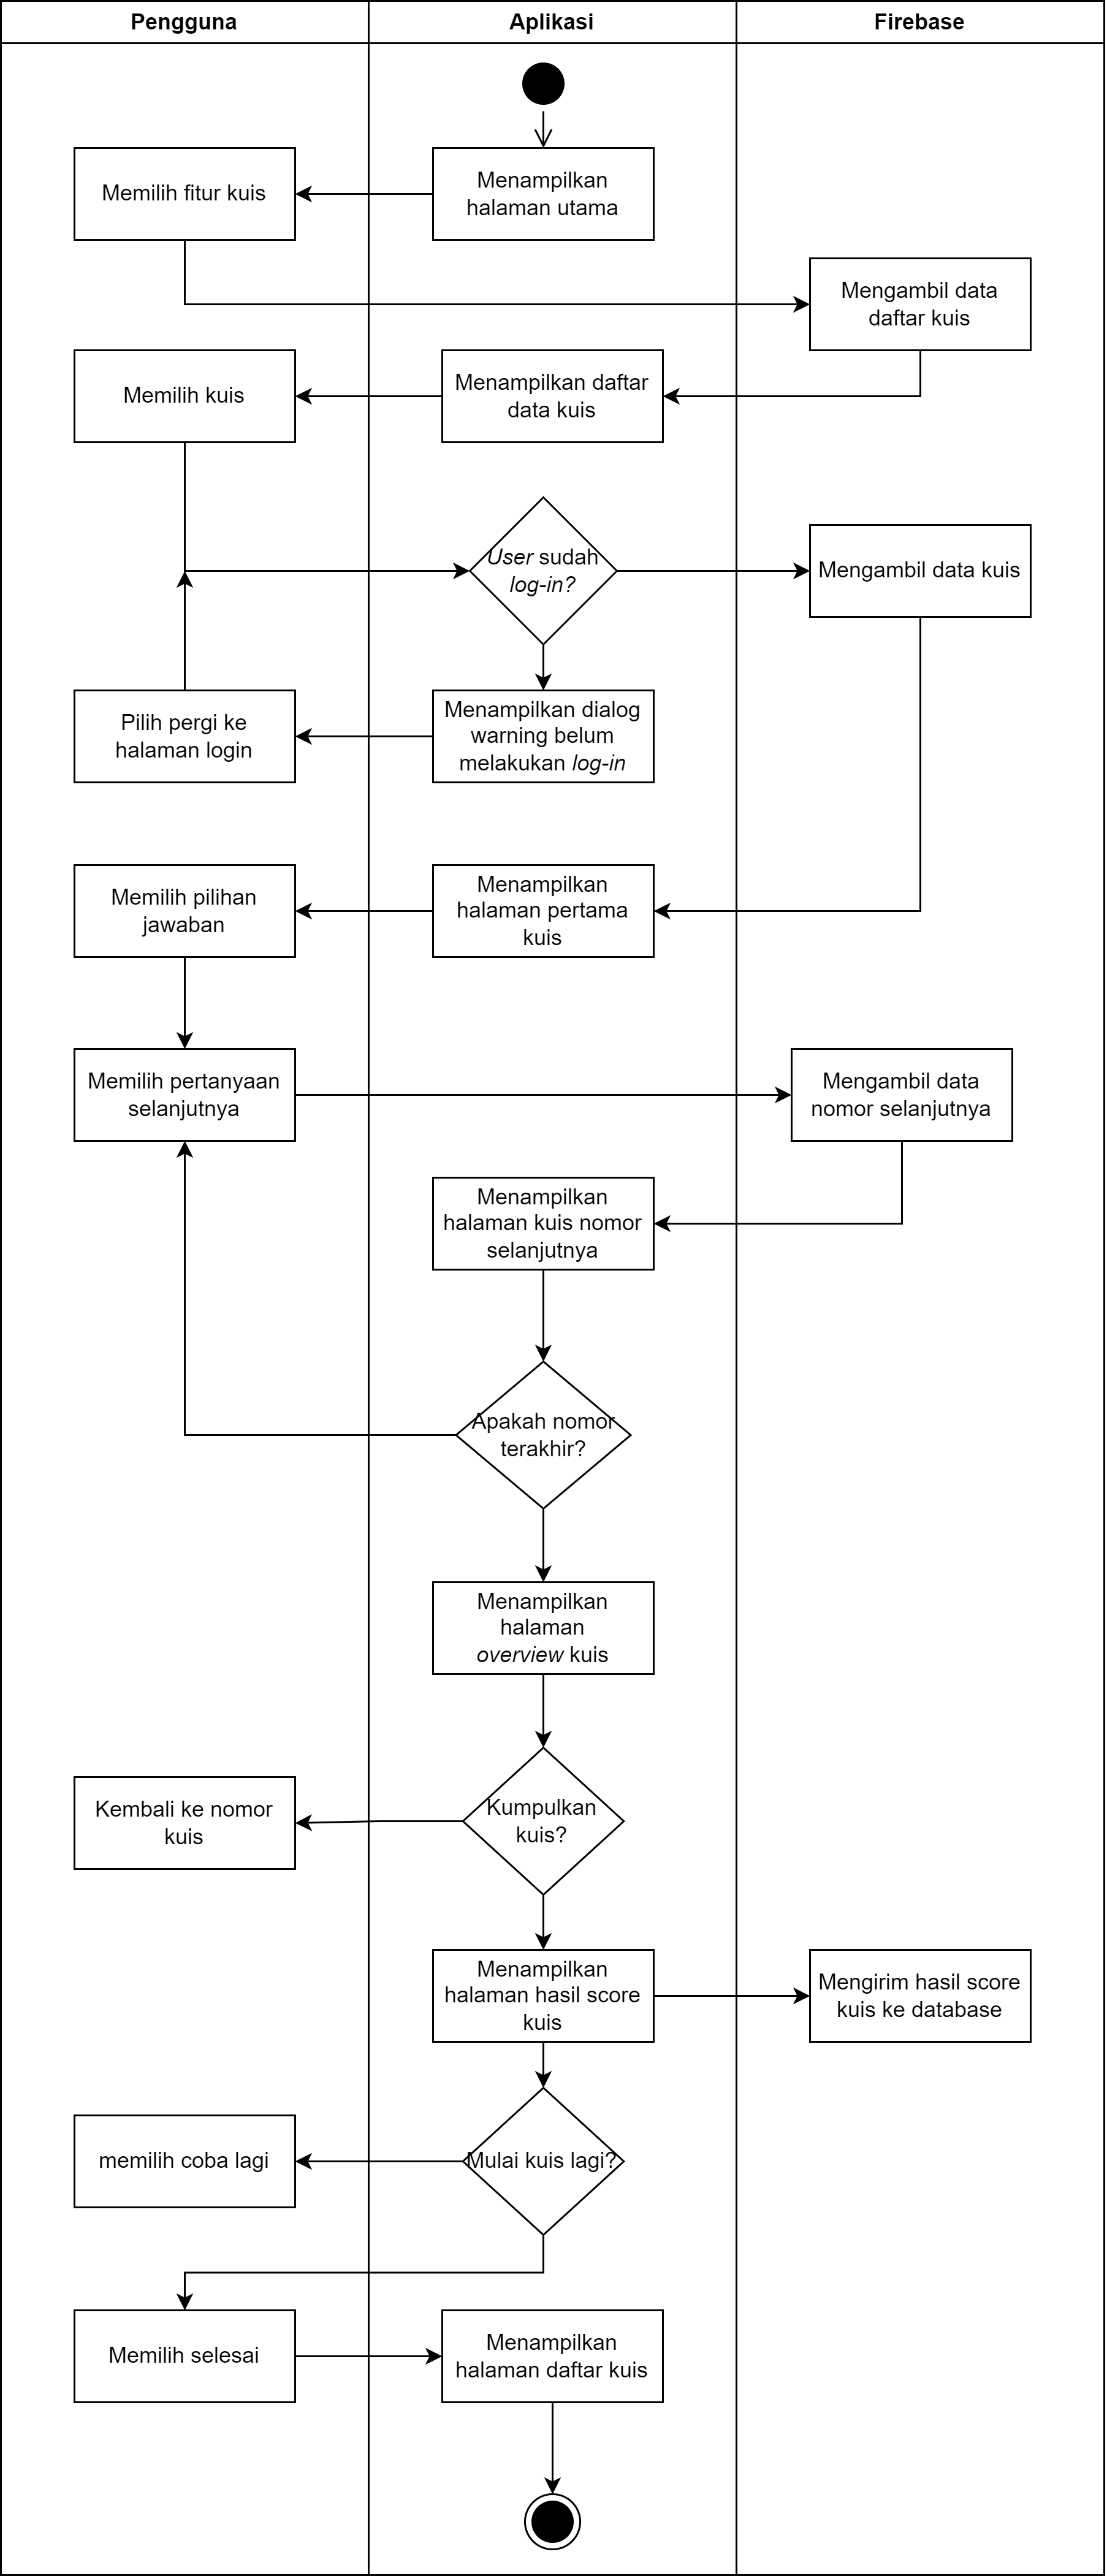
\includegraphics[width=0.6\textwidth]{contents/chapter-3/images/AD-kuis.png}
	\caption{\textit{Activity Diagram Quiz}}
	\label{fig:ActivityQuiz}
\end{figure}

Fitur kuis dalam aplikasi ini merupakan sebuah elemen mekanika permainan yang dapat dilakukan oleh pengguna. Selain itu, elemen kedua yang ada pada fitur ini ialah poin yang diperoleh pengguna jika sudah mengerjakan kuis.
Selain itu juga, fitur ini akan ditambahkan mekanika permainan untuk mengerjakan kuis dengan batas waktu tertentu menggunakan elemen \textit{time attack}. Elemen ini akan memberikan adrenalin pada pengguna ketika mengerjakan kuis.
Selain mekanika yang disebutkan, \textit{Replayability} pada fitur ini akan ditrapkan. Pengguna dapat mengerjakan kuis secara berulang ulang untuk lebih memahami materi yang disuguhkan.
\begin{figure}[H]
	\centering
	\begin{subfigure}[b]{0.3\textwidth}
		\centering
	  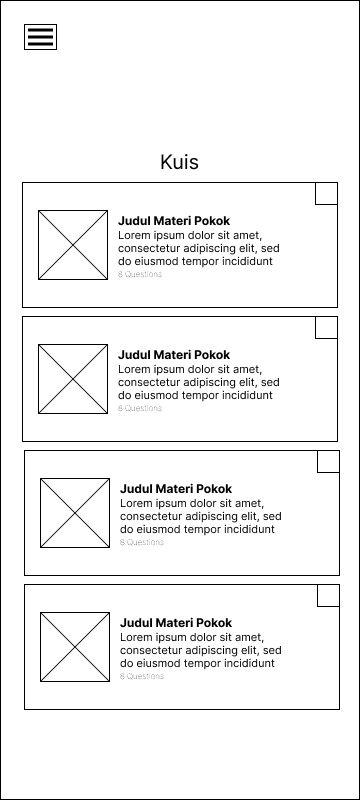
\includegraphics[width=\linewidth]{contents/chapter-3/images/MF-kuis.png}
	  \caption{\textit{Log-in page}}
	  \label{fig:midFi-Quiz}
	\end{subfigure}
	\begin{subfigure}[b]{0.3\textwidth}
		\centering
	  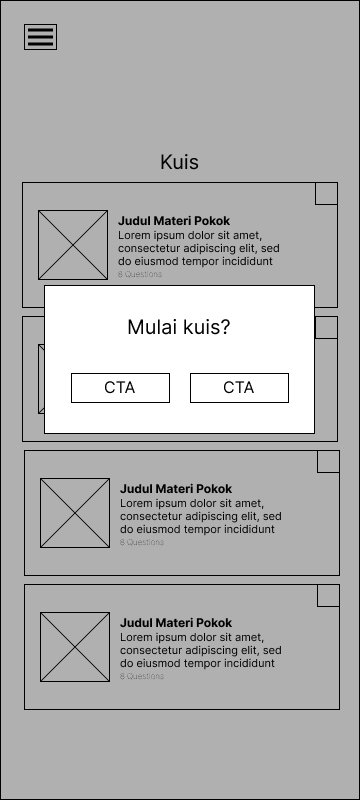
\includegraphics[width=\linewidth]{contents/chapter-3/images/MF-kuis-2.png}
	  \caption{\textit{Dialog Box} mulai kuis}
	  \label{fig:midfi-askQuiz}
	\end{subfigure}
	\begin{subfigure}[b]{0.3\textwidth}
		\centering
	  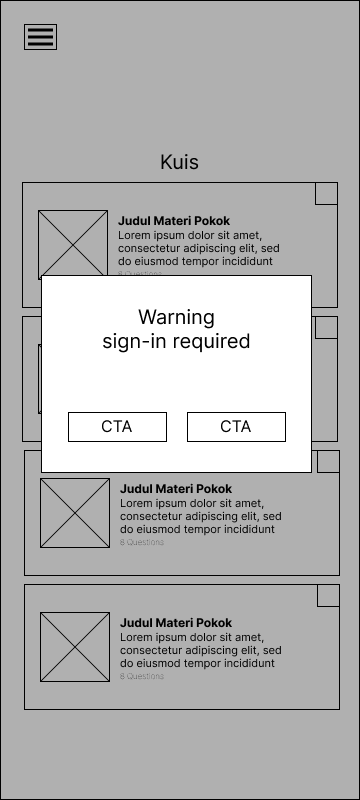
\includegraphics[width=\linewidth]{contents/chapter-3/images/MF-kuis-6.png}
	  \caption{\textit{Warning Dialog}}
	  \label{fig:midfi-quizWarning}
	\end{subfigure}
	\caption{\textit{Prototype} antarmuka halaman daftar kuis (fitur kuis)}
	\label{Fig:FeatureSetQuizList}
\end{figure}
Gambar \ref*{Fig:FeatureSetQuizList} merupaka prototype dari antarmuka halaman daftar kuis aplikasi.
Saat pergi ke halaman fitur kuis, aplikasi akan menampilkan deretan daftar kuis yang dapat dikerjakan oleh pengguna.
Saat akan memulai kuis, aplikasi akan memnanyakan terlebih dahulu dengan menampilkan \textit{Dialog box}.
Ketika pengguna memilih mengerjakan kuis, aplikasi akan menampilkan halaman pertama kuis yang berisi soal nomor pertama.

Gambar \ref*{Fig:FeatureSetQuiz} adalah desain \textit{prototype} untuk halaman kuis saat mengerjakan.
Gambar \ref*{fig:ActivityKuis} merupakan antarmuka dimanaa pengguna akan memilih jawaban dari pertanyaan kuis.
gambar \ref*{fig:ActivityKuis2} menunjukkan \textit{preview} kuis, dan gambar \textit{ActivityKuis3} menunjukkan hasil kuis seteleh selesai mengerjakan.
Elemen mekanika permainan dalam desain ini terdapat pada waktu yang terus berjalan saat pengguna memutuskan untuk mengerjakan kuis. Elemen ini akan disematkan pada halaman pengerjaan untuk menciptakan adrenalin pada penggunanya.
Selanjutnya ada elemen mekanika permainan poin yang akan diberikan berdasarkan jumlah jawaban yang benar dan waktu yang masih tersisa.
Poin ini juga yang akan menentukan dinamika permainan \textit{Leaderboard} yang akan dibandingkan dengan pengguna lain berdasarkan skor yang didapatkan.
\begin{algorithm}[H]
    \caption{Perhitungan poin}
	\begin{algorithmic}
		\Function{getPoints}{$remainSeconds$, $correctQuestionCount$, $quizPaperModel$}
		  \State $points \gets ((remainSeconds / quizPaperModel.timeSeconds) * 100) + (correctQuestionCount * 100)$
		  \State \Return $points.toStringAsFixed(2)$
		\EndFunction
		\end{algorithmic}
\end{algorithm}
Pergantian halaman antar nomor merupakan dinamika permainan yang diimplementasikan pada fitur ini, begitu juga dengan fitur \textit{overview} yang dapat secara bebas memilih nomor kuis yang ingin dikerjakan.
\begin{figure}[H]
	\centering
	\begin{subfigure}[b]{0.3\textwidth}
		\centering
	  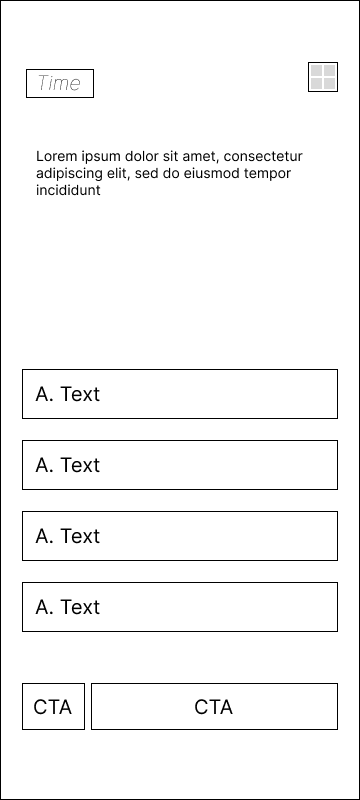
\includegraphics[width=\linewidth]{contents/chapter-3/images/MF-kuis-3.png}
	  \caption{Halaman kuis}
	  \label{fig:ActivityKuis}
	\end{subfigure}
	\begin{subfigure}[b]{0.3\textwidth}
		\centering
	  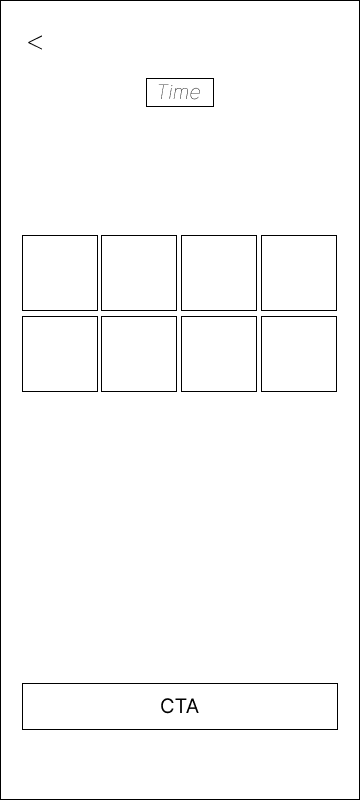
\includegraphics[width=\linewidth]{contents/chapter-3/images/MF-kuis-4.png}
	  \caption{\textit{Overview} kuis}
	  \label{fig:ActivityKuis2}
	\end{subfigure}
	\begin{subfigure}[b]{0.3\textwidth}
		\centering
	  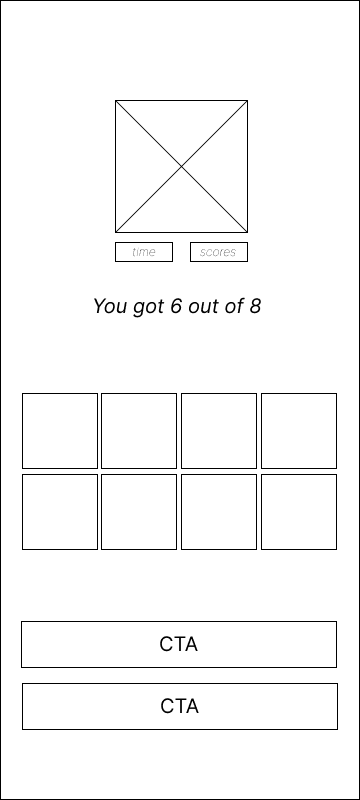
\includegraphics[width=\linewidth]{contents/chapter-3/images/MF-kuis-5.png}
	  \caption{Hasil kuis}
	  \label{fig:ActivityKuis3}
	\end{subfigure}
	\caption{\textit{Prototype} antarmuka halaman kuis}
	\label{Fig:FeatureSetQuiz}
\end{figure}
\subsubsection{\textit{Feature set : Leaderboard}}
Fitur selanjutnya yang berhubungan denganfitur kuis ialah fitur \textit{Leaderboard}. 
Fitur ini memungkinkan untuk mengurutkan urutan perolehan poin berdasarkan jumlah poin yang didapatkan pada masing-masing kuis.
Fitur ini pada kerangka kerja gamifikasi termasuk ke dalam kategori dinamika permainan dimana pengguna bisa berkompetisi untuk mendapatkan skor paling tinggi.
Skenario digambarkan pada gambar \ref*{Fig:ActivityLeaderboard}.
\begin{figure}[H]
	\centering
	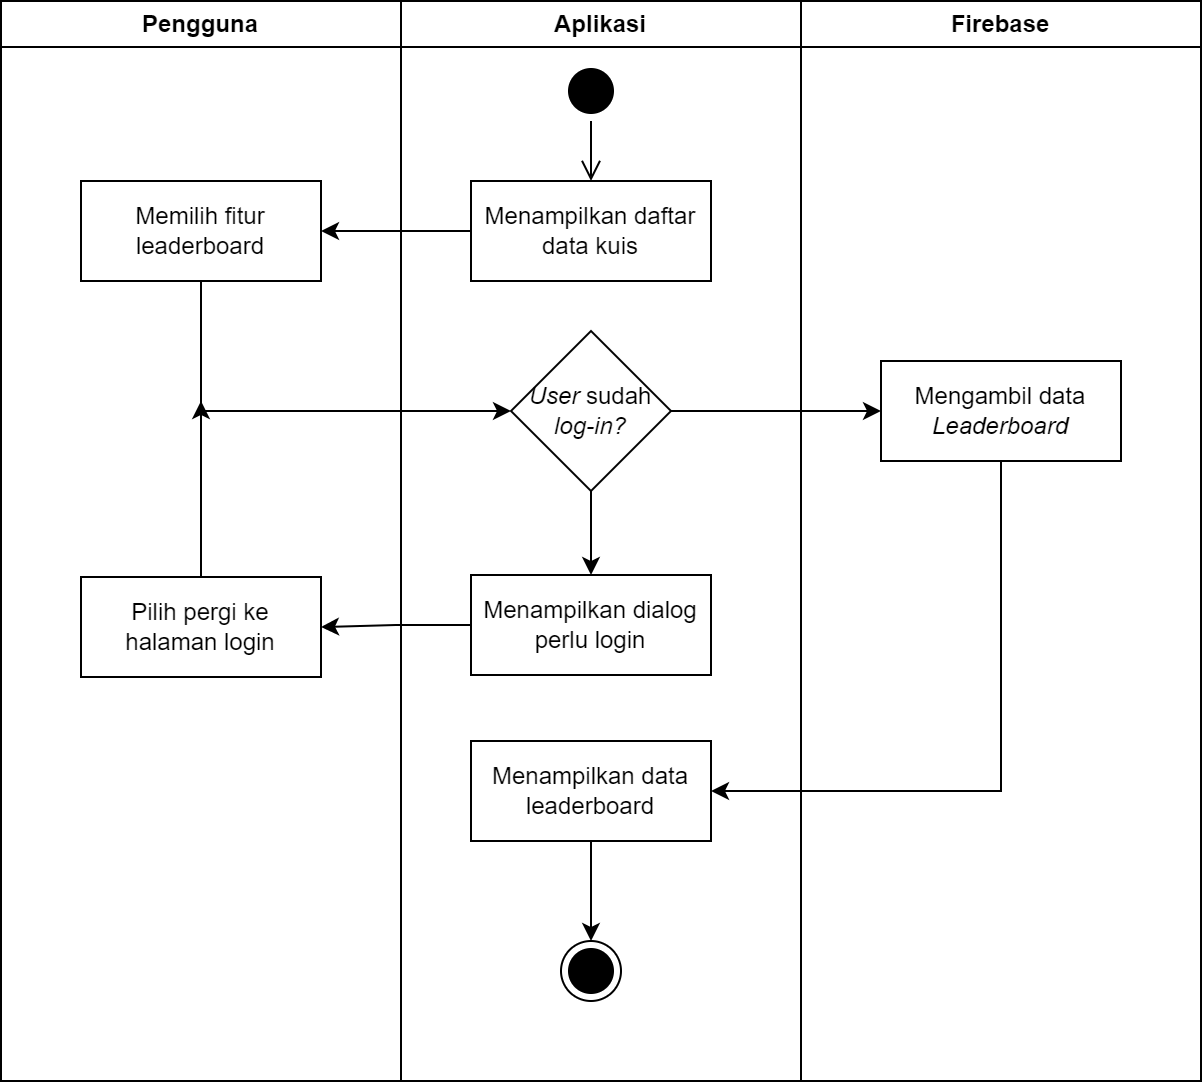
\includegraphics[width=0.65\textwidth]{contents/chapter-3/images/AD-leaderboard.png}
	\caption{\textit{Activity Diagram} fitur \textit{Leaderboard}}
	\label{Fig:ActivityLeaderboard}
\end{figure}
Kemudian, gambar \ref*{Fig:ActivityLeaderboard2} adalah \textit{prototype} halaman \textit{leaderboard}.
Fitur ini menampilkan nama pengguna secara berurutan berdasarkan skor yang didapatkan.
Fitur ini akan mengurutkan pengguna pada setiap kuis yang dikerjakan, dengan demikian setiap kuis akan memiliki pengguna dengan skor tertinggi yang berbeda beda.
\begin{figure}[H]
	\centering
	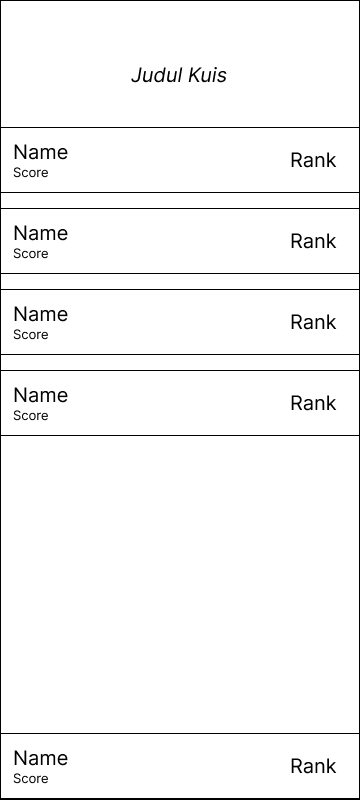
\includegraphics[width=0.3\textwidth]{contents/chapter-3/images/MF-leaderboard.png}
	\caption{\textit{Prototype} antarmuka fitur \textit{Leaderboard}}
	\label{Fig:ActivityLeaderboard2}
\end{figure}
\subsubsection{\textit{Feature set :} Materi}

Sama seperti fitur kuis, fitur materi juga merupakan salah satu elemen mekanika permainan dalam aplikasi ini.
Mode materi ini memungkinkan kita mendapatkan materi pembelajaran mengenai \textit{Clinical Decision Support System}.
Pada fitur ini, dinamika permainan yang dialami pengguna adalah memahami materi secara berurutan. Elemen ini didukung dengan estetika permainan fitur \textit{Lock Part}.
Fitur ini memungkinkan materi selanjutya tetap terkunci sebelum materi sebelumnya selesai dibuka. Skenario fitur ini digambarkan pada gamabar \ref*{Fig:ActivityMateri} dan didesain antarmukanya pada gambar \ref*{fig:ActivityMateri2}
\begin{figure}[H]
	\centering
	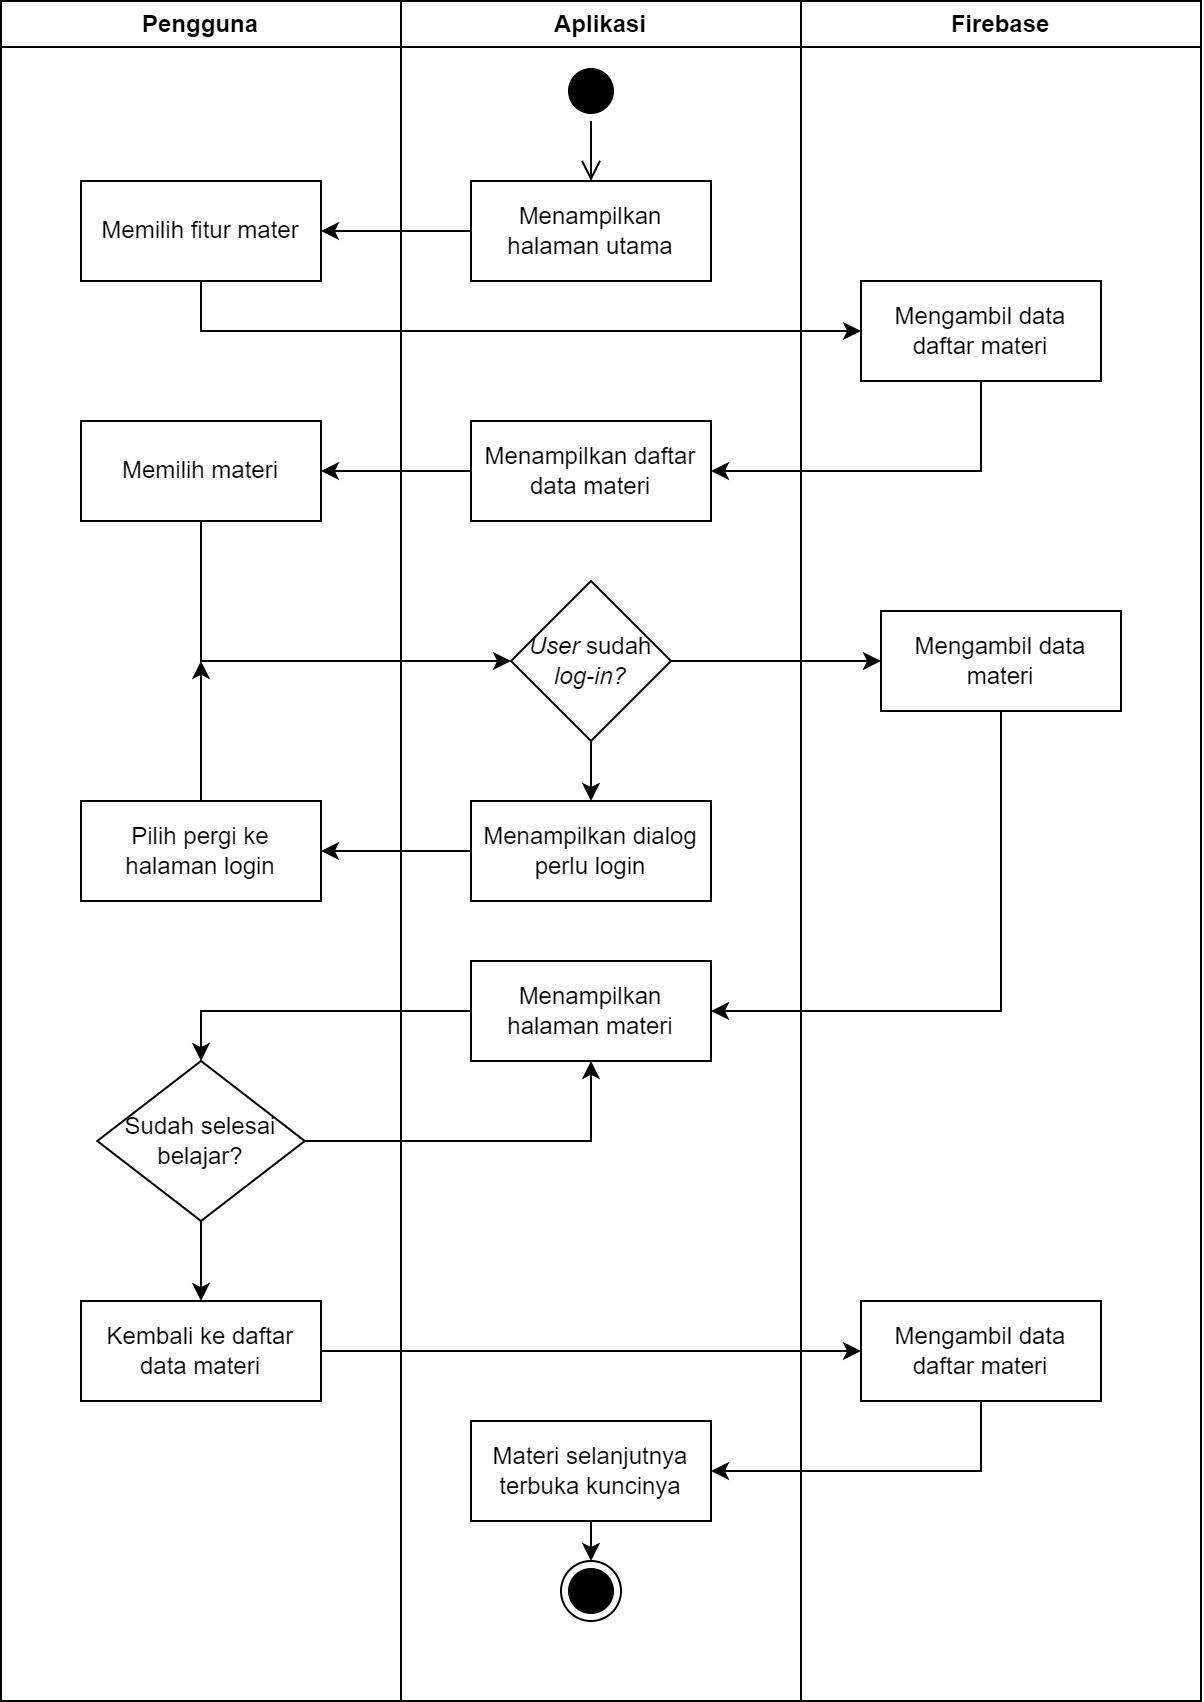
\includegraphics[width=0.7\textwidth]{contents/chapter-3/images/AD-materi.png}
	\caption{\textit{Activity Diagram} fitur materi }
	\label{Fig:ActivityMateri}
\end{figure}

Gambar \ref*{Fig:FeatureSetSubject} adalah antarmuka fitur materi dari aplikasi ini.
Fitur materi ini secara umum adalah menampilkan file pdf yang didesain semenarik mungkin untuk meningkatkan estetika permainan.
\begin{figure}[H]
	\centering
	\begin{subfigure}[b]{0.3\textwidth}
		\centering
	  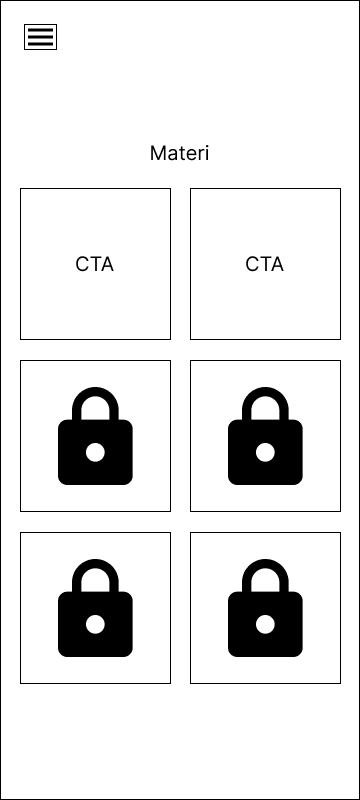
\includegraphics[width=\linewidth]{contents/chapter-3/images/MF-materi.png}
	  \caption{Daftar materi}
	  \label{fig:ActivityMateri2}
	\end{subfigure}
	\begin{subfigure}[b]{0.3\textwidth}
		\centering
	  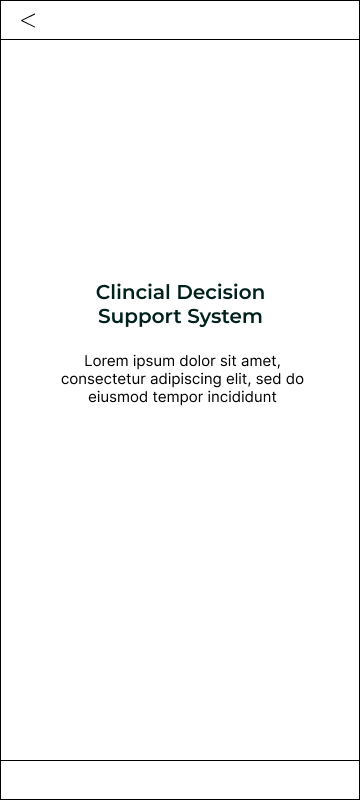
\includegraphics[width=\linewidth]{contents/chapter-3/images/MF-materi-2.png}
	  \caption{Halaman Materi}
	  \label{fig:ActivityMateri3}
	\end{subfigure}
	\begin{subfigure}[b]{0.3\textwidth}
		\centering
	  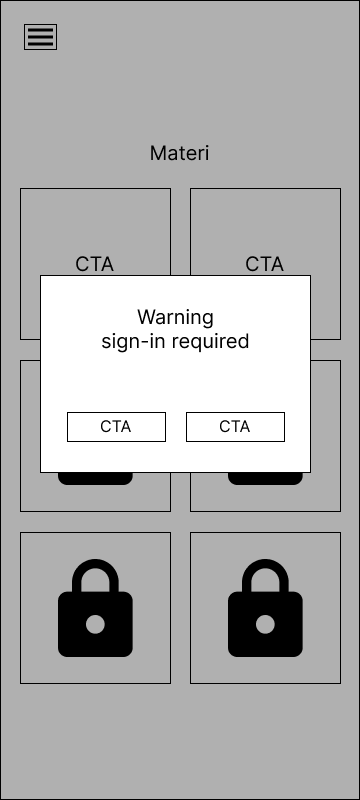
\includegraphics[width=\linewidth]{contents/chapter-3/images/MF-materi-4.png}
	  \caption{Halaman Materi}
	  \label{fig:ActivityMateri}
	\end{subfigure}
	\caption{\textit{Prototype} antarmuka halaman fitur materi}
	\label{Fig:FeatureSetSubject}
\end{figure}
\subsubsection{\textit{Feature set : Achievement}}

Ada juga fitur penghargaan pada aplikasi ini. Skenario fitur ini digambarkan pada gambar \ref*{Fig:ActivityProfiil}
\begin{figure}[H]
	\centering
	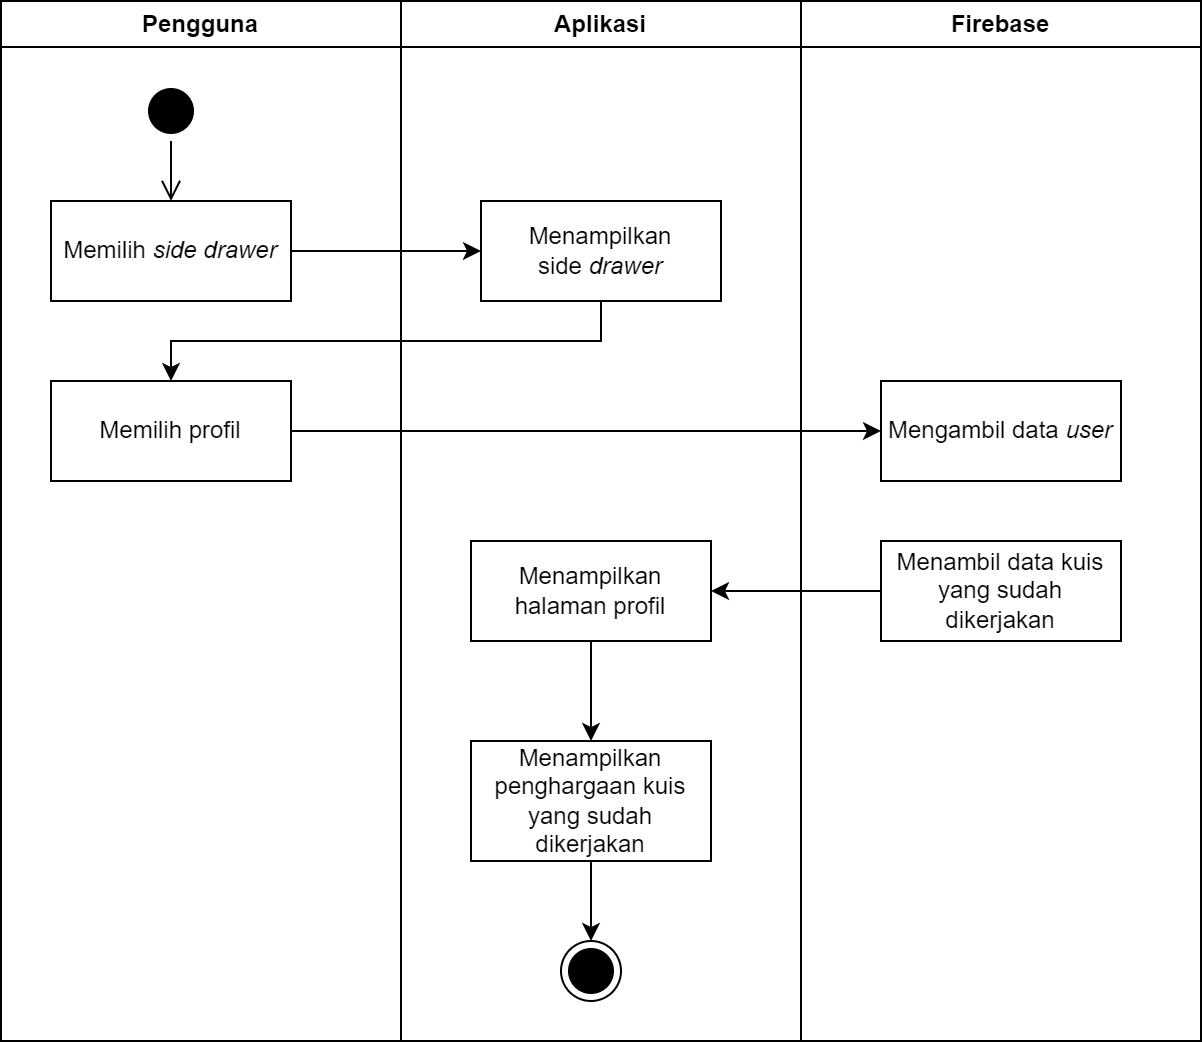
\includegraphics[width=0.7\textwidth]{contents/chapter-3/images/AD-profil.png}
	\caption{\textit{Activity Diagram} fitur \textit{Achievement}}
	\label{Fig:ActivityProfiil}
\end{figure}
Fitur penghargaan akan terdapat pada halaman profil aplikasi.
Fitur ini merupakan salah satu mekanika permainan yang diimplementasikan pada aplikasi ini.
Penghargaan yang didapat merupakan penghargaan setiap kuis yang telah diselesaikan.
Setiap kuis yang sudah dikerjakan, penghargaan akan ditambahkan pada halaman profil.
Penghargaan akan menampilkan nama kuis yang sudah dikerjakan, jumlah skor, dan jumlah jawaban yag benar.
\textit{Prototype} desain ada pada gambar \ref*{Fig:ActivityProfil2}
\begin{figure}[H]
	\centering
	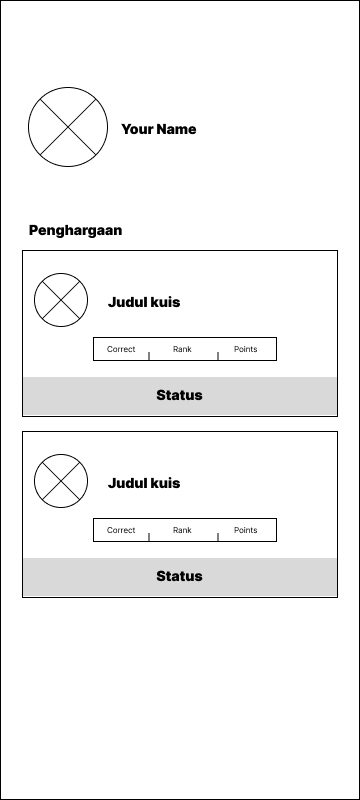
\includegraphics[width=0.3\textwidth]{contents/chapter-3/images/MF-Profil.png}
	\caption{\textit{Prototype} antarmuka pada fitur \textit{Achievement}}
	\label{Fig:ActivityProfil2}
\end{figure}
\subsection{\textit{Build by Feature}}
Tahap \textit{Build by Feature} merupakan tahap \textit{coding} dan implementasi tiap fitur pada \textit{feature set}.
\textit{feature set} dibagi berdasarkan \textit{Main Activity}. Pengembangan dialakukan secara berurutan dari fitur ke fitur.
Jika da kegagalan pada tahap ini, maka pengembangan fitur akan kembali ke tahap desain.
Tahap pengembangan ini disertai dengan pengembangan gamifikasi yang sudah diimplementasikan pada tahap desain.

Aplikasi ini akan dikembangkan pada platform mobile Android menggunakan \textit{Software Development Kit Flutter}, dan \textit{Firebase}.
\textit{Flutter} dan \textit{Firebase}. \textit{Flutter} dipilih karena pengebangannya cukup mudah dan familiar karena mirip dengan pengembangan \textit{web}.
Untuk \textit{Firebase} sendiri dipilih karena layanan tersebut sudah mencakup layanan \textit{back-end} dan \textit{database} sehingga memudahkan penulis dalam pengembangannya.
Tools yang digunakan antara lain \textit{Visual Studio Code} sebagai \textit{Text Editor}, \textit{Android Emulator} pada\textit{Android Studio} untuk mendebug kode.
\subsection{Menguji Fungsionalitas Aplikasi \textit{Black Box Testing}}
pengujian ini diujikan untuk memastikan keseluruhan functional requirements sudah berjalan seusai dengan harapan dan kemudian dapat diujikan langsung ke pengguna
\begin{table}[H]
	\centering
	\caption{Daftar fitur dan kriteria yang diharapkan}
	\begin{tabular}{|m{1cm}|p{0.45\textwidth}|p{0.45\textwidth}|}
		\hline
		\centering\textbf{ID} & \centering\textbf{Fitur} & \multicolumn{1}{m{0.45\textwidth}|}{\centering \textbf{Kriteria}} \\
		\hline
		F-01 &Menampilkan halaman Sign-in & Aplikasi mampu menampilkan halaman \textit{sign-in} \\
		\hline
		F-02 &Mencatat \textit{user} baru ketika melakukan \textit{Sign-in} pertama & Aplikasi dapat mencatat \textit{user} baru ketika melakukan \textit{Sign-in} pertama dan mengirimkannya ke database\\
		\hline
		F-03 &Aplikasi dapat memberikan akses pengguna ketika pengguna sudah terdaftar& Pengguna dapat menggunakan fitur aplikasi\\
		\hline
		F-04 &Menampilkan halaman \textit{On Boarding} jika \textit{user} belum terdaftar & Aplikasi mampu menampilkan halaman \textit{On Boarding} jika \textit{user} belum terdaftar  \\
		\hline
		F-05&Menampilkan halaman utama aplikasi& Ketika sudah \textit{sign-in}, penguna dapat mengakses halalman utama \\
		\hline
		F-06&Menampilkan \textit{side drawer}& Aplikasi mempu menampilkan \textit{side drawer} pada sebelah kiri aplikasi\\
		\hline
		F-07&\textit{Dialog box Sign Up} jika memilih fitur, tapi \textit{user} belum terdaftar& Jika pengguna belum \textit{sign-in}, aplikasi menampilkan dialog box \\
		\hline
		F-08&Memilih fitur kuis, materi, dan profil& Aplikasi mampu menampilkan semua fitur yang ada\\
		\hline
		F-09 &Menampilkan halaman daftar materi yang tersedia& Aplikasi mampu menampilkan halaman fitur materi yang berisi daftar materi \\
		\hline
		F-10&Menampilkan materi yang dipilih & Aplikasi mampu menampilkan materi yang dipilih\\
		\hline
		F-11&Keluar dari materi yang dipilih& aplikasi mampu keluar dari aplikasi yang dipilih\\
		\hline
		F-12&Fitur kunci materi jika materi sebelumnya belum dibaca& Aplikasi akan mengunci file materi jika materi sebelumnya belum pernah dibuka, dan membuka jika materi seblumnya sudah pernah dibuka. \\
		\hline
	\end{tabular}
\end{table}
\newpage
\begin{table}[H]
	\begin{tabular}{|m{1cm}|p{0.45\textwidth}|p{0.45\textwidth}|}
		\hline
		\centering\textbf{ID} & \centering\textbf{Fitur} & \multicolumn{1}{m{0.45\textwidth}|}{\centering \textbf{Kriteria}} \\
		\hline
		F-13&Keluar dari halaman daftar materi dan kembali ke halaman utama& Aplikasi mampu menutup fitur materi dan kembali ke halaman utama \\
		\hline
		F-14 &Menampilkan halaman daftar kuis&  Aplikasi mampu menampilkan halaman fitur kuis yang berisi daftar kuis\\
		\hline
		F-15&Menampilkan halaman kuis yang dipilih&  Aplikasi mampu menampilkan halaman kuis yang dipilih \\
		\hline
		F-16&Memilih salah satu jawaban kuis berbasis pilihan ganda& Aplikasi mampu meilih dan menyimpan jawaban \\
		\hline
		F-17&Menampilkkan halaman kuis nomor selanjutnya& Aplikasi akan menampilkan halaman kuis selanjutnya\\
		\hline
		F-18&Menampilkan halaman kuis nomor sebelumnya& Aplikasi akan menampilkan halaman kuis sebelumnya \\
		\hline
		F-19&Menampilkan ringkasan kuis& Aplikasi akan menampilkan halaman ringkasan kuis  \\
		\hline
		F-20&Menyelesaikan kuis& Aplikasi dapat menutup halaman utama kuis, menghitung jawaban yang benar, dan mengirim hasilya ke database \\
		\hline
		F-21&Mendapatkan skor kuis& Aplikasi akan  menghitung jawaban yang benar dan menampilkan skor hasil kuis \\
		\hline
		F-22&Mencatat skor kuis& Aplikasi dapat mengirimkan hasil kuis ke database\\
		\hline
		F-23&Menampilkan warna merah untuk jawaban yang salah dan warna hijau untuk jawaban yang benar dalam ulasan kuis& Aplikasi mampu Menampilkan warna merah untuk jawaban yang salah dan warna hijau untuk jawaban yang benar dalam ulasan kuis  \\
		\hline
		F-24&Memeriksa 1 per 1 jawaban kuis setelah mendapatkan skor& Aplikasi mampu menampilkan halaman soal kuis sesuai dengan indeks yang dipilih \\
		\hline
		F-25&Mengerjakan kembali kuis& Aplikasi mampu menampilkan halaman pertama kuis dan memulai dari awal\\
		\hline
		F-26&Menutup halaman kuis dan kembali ke halaman daftar kuis& Aplikasi mampu menutup halaman kuis dan menampilkan halaman daftar kuis \\
		\hline
	\end{tabular}
\end{table}
\newpage
\begin{table}[H]
	\begin{tabular}{|m{1cm}|p{0.45\textwidth}|p{0.45\textwidth}|}
		\hline
		\centering\textbf{ID} & \centering\textbf{Fitur} & \multicolumn{1}{m{0.45\textwidth}|}{\centering \textbf{Kriteria}} \\
		\hline
		F-27&Menutup halaman daftar kuis dan kembali ke halaman utama& Aplikasi mampu menutup halaman fitur daftar kuis dan kembali ke halaman utama \\
		\hline
		F-28 &Menampilkan halaman \textit{Leaderboard} untuk kuis yang dipilih &Aplikasi mampu menampilkan leaderboard untuk setiap indeks yang dipilih pada kuis \\
		\hline
		F-29&Menampilkan hasil skor kuis pribadi yang sudah dikerjakan& Aplikasi menampilkan hasil skor pribadi pada halaman Leaderboard\\
		\hline
		F-30&Menampilkan urutan skor dari yang tertinggi hingga terendah& Aplikasi akan mengurutkan rangking pengguna berdasarkan skor kuis \\
		\hline
		F-31&Menutup halaman leaderboard dan kembali ke halaman daftar kuis& Aplikasi mampu menutup halaman leaderboard dan menampilkan halaman daftar kuis\\
		\hline
		F-32 &Menampilkan halaman profil& Aplikasi mampu menampilkan halaman profil \\
		\hline
		F-33&Menampilkan penghargaan yang ada dalam halaman profil& Aplikasi mampu menampilkan daftar penghargaan dari kuis yang sudah dikerjakan \\
		\hline
		F-34&Menampilkan hasil scroe dari setiap kuis yang sudah dikerjakan& Aplikasi mampu maenampilkan hasil skor kuis dalam penghargaan kuis\\
		\hline
		F-35&Menutup halaman profil dan kembali ke halaman utama aplikasi&Aplikasi mampu menutup halaman profil dan menampikan halaman utama \\
		\hline
		F-36 &Menghentikan pemberian akses pengguna ketika pengguna sudah terdaftar& Aplikasi mampu mengeluarkan akses aplikasi apda akun terkait\\
		\hline
	\end{tabular}
\end{table}
\subsection{Pengujian Aplikasi}
Pada tahap ini, aplikasi yang sudah dikembangkan dan diujikan fungsionallitasnya kemudian akan diujikan juga kebergunaanya pada pengguna nyata.
Proses pengujiannya ini menggunakan \textit{System Usability Testing(SUS)} untuk mengukur kebergunaan, dan \textit{User Experience Questionnaire(UEQ)} untuk mengukur feedback pengalaman yang didapatkan setelah menggunakan aplikasi.
\textit{System Usability Testing(SUS)} dipilih karena pengujian ini dapat mengujikan aplikasi yang dikembangkan sudah layak digunakan atau belum.
Untuk mengukur efek dari aplikasi ini,\textit{User Experience Questionnaire(UEQ)} dipilih karena pengujian ini mampu memberikan nilai Efektivitas yang sesuai dengan tujuan gamifikasi sendiri. 
Untuk tahapan pengujian akan dilakukan seperti pada gambar 
populasi yang diambil dari pengujiannya ini adalah mahasiswa yang sedang atau ingin mempelajari ilmu dasar \textit{Clinical Decision Support System}.
Pada pengujian ini, mayortas populasinya ialah mahasiswa teknik biomedis DTETI UGM.
Responden akan membaca kertas instruksi yang berisi poin-poin \textit{objective} yang dapat dilakukan pada aplikasi.
Kemudian responden akan menguji coba aplikasi dengan mengerjakan seluruh \textit{objective} yang ada. Responded diberi waktu 10 menit untuk mengerjakan seluruh \textit{objective}.
Setelah itu pengujian pertama responden akan mengisikan formulir \textit{System Usability Testing(SUS)} untuk menilai kebergunaan aplikasinya, dan dilanjutkan dengan mengisi formulir \textit{User Experience Questionnaire(UEQ)} untuk menilai pengalaman.
\subsection{Analisis Hasil Pengujian}
Hasil kuesioner SUS dan UEQ yang didapat kemudian dilakukan 
perhitungan menggunakan rumus dan alat yang sesuai untuk mendapatkan hasil 
uji. Hal ini untuk menentukan apakah aplikasi sudah cukup bagus atau perlu ada 
perbaikan kedepan. 
% Bagian ini membahas pertimbangan etis penelitian dan [potensi] masalah serta
% keterbatasannya. Jika menyangkut penelitian dengan makhluk hidup, maka dibutuhkan adanya \textit{ethical clearance}, di bagian ini hal itu akan dibahas. Demikian juga tentang keterbatasan ataupun masalah yang akan timbul.
